%!TEX root = ../../book_ML.tex
\chapter{Mạng neuron đa tầng và lan truyền ngược}
\label{cha:mlp}
 
% Vì chương này sử dụng khá nhiều công thức toán, bạn đọc được khuyến khích đọc \href{http://machinelearningcoban.com/math/#luu-y-ve-ky-hieu}{Lưu ý về ký hiệu toán học}. 
 
 
\section{Giới thiệu}
 
% Bài toán \href{http://machinelearningcoban.com/2016/12/27/categories/#supervised-learning-hoc-co-giam-sat}{Supervised Learning}, nói một cách ngắn gọn, là việc đi tìm một hàm số để với mỗi \textit{input}, ta sử dụng hàm số đó để dự đoán \textit{output}. Hàm số này được xây dựng dựa trên các cặp dữ liệu $(\mathbf{x}_i, \mathbf{y}_i)$ trong \textit{training set}. Nếu \textit{đầu ra dự đoán} (predicted output) gần với \textit{đầu ra thực sự} (true output) thì đó được gọi là một thuật toán tốt (nhưng khi \textit{đầu ra dự đoán quá giống với đầu ra thực sự} thì không hẳn đã tốt, mời bạn xem thêm Chương Overfitting.). 
 
 
\subsection{Perceptron cho các hàm logic cơ bản}
 
Chúng ta cùng xét khả năng của perceptron (PLA) trong bài toán biểu
diễn các hàm logic nhị phân: NOT, AND, OR, và XOR\footnote{đầu ra bằng \pythoninline{True}
nếu và chỉ nếu hai đầu vào logic khác nhau.}. Để có thể sử dụng PLA với
đầu ra là 1 hoặc -1, ta quy ước \pythoninline{True = 1} và \pythoninline{False = -1} ở đầu ra. Quan sát hàng trên của Hình~\ref{fig:14_1}, các điểm
hình vuông là các điểm có nhãn bằng 1, các điểm hình tròn là các
điểm có nhãn bằng -1. Hàng dưới của Hình~\ref{fig:14_1} là các mạng
perceptron với những hệ số tương ứng.
\begin{figure}[t]
 \vspace{.1in}
\centering
    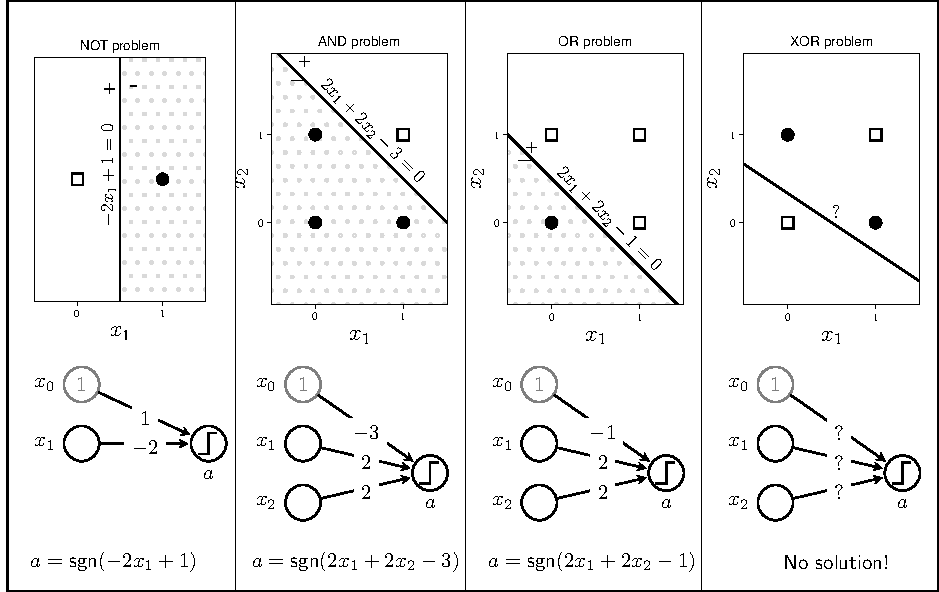
\includegraphics[width = \textwidth]{Chapters/05_NeuralNetworks/14_mlp/latex/logic_nn.pdf}
    \caption[]{Biểu diễn các hàm logic cơ bản sử dụng perceptron.}
    \label{fig:14_1}
\end{figure}
Nhận thấy rằng với bài toán NOT, AND, và OR, dữ liệu hai lớp là tách biệt tuyến, vì vậy ta có thể tìm được các hệ số cho mạng perceptron giúp biểu diễn
chính xác mỗi hàm số. Chẳng hạn với hàm NOT, khi $x_1 = 0$ (False), ta có $a =
\text{sgn}(-2 \times 0+1) = 1$ (True); khi $x_1 = 1$, $a = \text{sgn}(-2\times 1 + 1) =
-1$. Trong cả hai trường hợp, đầu ra dự đoán đều giống đầu ra thực sự. Bạn
đọc có thể tự kiểm chứng các hệ số với hàm AND và OR.

\subsection{Biểu diễn hàm XOR với nhiều perceptron}
Đối với hàm XOR, vì dữ liệu không tách biệt tuyến tính nên không thể biểu diễn
bằng một perceptron. Nếu thay perceptron bằng hồi quy logistic ta cũng không tìm
được các hệ số thỏa mãn, vì về bản chất, hồi quy logistic hay cả hồi quy softmax
chỉ tạo ra các ranh giới tuyến tính. Như vậy, các mô hình mạng neuron đã biết
không thể biểu diễn được hàm số logic đơn giản này.
 
 
 
\begin{figure}[t]
\centering
    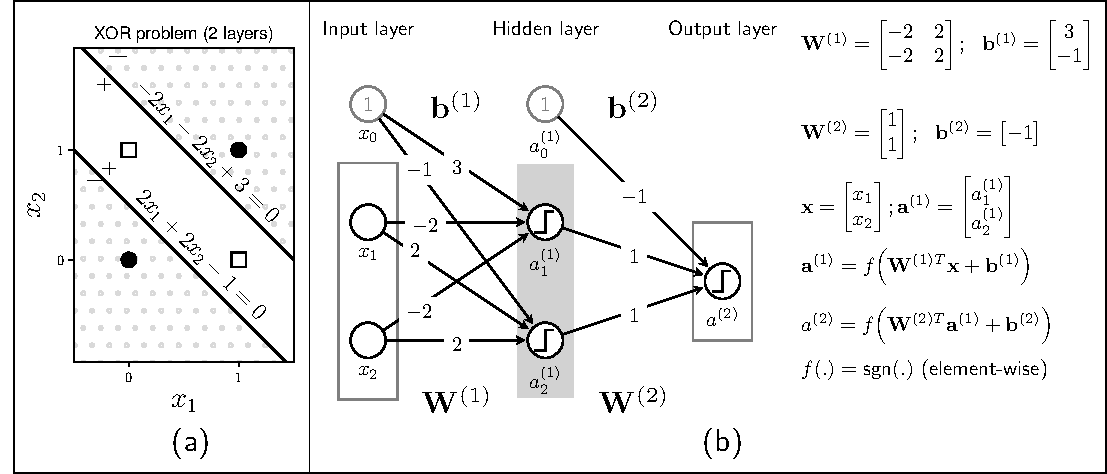
\includegraphics[width = \textwidth]{Chapters/05_NeuralNetworks/14_mlp/latex/xor_nn.pdf}
    \caption[]{Ba perceptron biểu diễn hàm XOR.}
    \label{fig:14_2}
\end{figure}

Nhận thấy rằng nếu cho phép sử dụng hai đường thẳng, bài toán biểu diễn hàm XOR
có thể được giải quyết như Hình \ref{fig:14_2}. Các hệ số tương ứng với hai
đường thẳng trong Hình~\ref{fig:14_2}a được minh họa trên Hình~\ref{fig:14_2}b. Đầu ra $a_1^{(1)}$ bằng 1
với các điểm nằm về phía (+) của đường thẳng $3 -2x_1 -2x_2 = 0$, bằng -1 với
các điểm nằm về phía (-). Tương tự, đầu ra $a_2^{(1)}$ bằng 1 với các điểm nằm về phía
(+) của đường thẳng $-1 +2x_1 + 2x_2 = 0$. Như vậy, hai đường thẳng ứng với hai
perceptron này tạo ra hai đầu ra tại các nút $a_1^{(1)}, a_2^{(1)}$. Vì hàm XOR
chỉ có một đầu ra nên ta cần thêm một bước nữa: coi $a_1, a_2$ như là đầu
vào của một perceptron khác. Trong perceptron mới này, đầu vào là các nút ở giữa
(cần nhớ giá trị tương ứng với hệ số điều chỉnh luôn có giá trị bằng 1), đầu ra là nút bên phải. Các hệ số
được cho trên Hình~\ref{fig:14_2}b. Kiểm tra lại một chút, với các điểm hình
vuông (Hình~\ref{fig:14_2}a), $a^{(1)}_1 = a^{(1)}_2 = 1$, khi đó $a^{(2)}
= \text{sgn}(-1 +1 + 1) = 1$. Với các điểm hình tròn, vì $a^{(1)}_1 =
-a^{(1)}_2$ nên $a^{(2)} = \text{sgn}(-1 + a^{(1)}_1 + a^{(1)}_2) =
\text{sgn}(-1) = -1$. Trong cả hai trường hợp, đầu ra dự đoán đều giống với đầu
ra thực sự. Như vậy, ta sẽ biểu diễn được hàm XOR nếu sử dụng ba perceptron. Ba perceptron kể trên được
xếp vào hai \textit{tầng} ({layers}). Ở đây, đầu ra của tầng thứ nhất chính là
đầu vào của tầng thứ hai. Tổng hợp lại ta được một mô hình mà ngoài tầng đầu
vào và đầu ra, ta còn có một tầng ở giữ có nền xám. 

Một mạng neuron với nhiều hơn hai tầng còn được gọi là \textit{mạng neuron đa tầng} (multi-layer neural network) hoặc \textit{perceptron đa tầng}(multilayer perceptron -- MLP). Tên gọi
\textit{perceptron} ở đây có thể gây nhầm lẫn\footnote{Geofrey Hinton,
\textit{phù thuỷ Deep Learning}, từng thừa nhận trong khoá học ``Neural Networks
for Machine Learning'' (\url{https://goo.gl/UfdT1t}) rằng ``Multilayer Neural
Networks should never have been called Multilayer Perceptron. It is partly my
fault, and I'm sorry.''.}, vì cụm từ này để chỉ mạng neuron nhiều tầng 
và mỗi tầng không nhất thiết là một hoặc
nhiều perceptron. Thực chất, perceptron rất hiếm khi được sử dụng trong các mạng neuron đa tầng. Hàm kích hoạt thường là các hàm phi tuyến khác thay vì hàm
sgn.

% \index{hàm kích hoạt -- activation function}

Một mạng neuron đa tầng có thể xấp xỉ mối quan hệ giữa
các cặp quan hệ $(\bx, \by)$ trong tập huấn luyện bằng một hàm số có dạng 
\begin{equation}
    \by \approx g^{(L)}\left(g^{(L-1)}\left(\dots
    (g^{(2)}(g^{(1)}(\bx)))\right)\right).
\end{equation}
Trong đó, tầng thứ nhất đóng vai trò như hàm $\ba^{(1)} \triangleq
g^{(1)}(\bx)$;
tầng thứ hai đóng vai trò như hàm $\ba^{(2)} \triangleq g^{(2)}(g^{(1)}(\bx)) =
f^{(2)}(\ba^{(1)})$,... 

Trong phạm vi cuốn sách, chúng ta quan tâm tới các tầng đóng vai trò như các
hàm có dạng
\begin{equation}
    g^{(l)}(\ba^{(l-1)}) = f^{(l)}(\bW^{(l)T}\ba^{(l-1)} + \bb^{(l)})
\end{equation}
với $\bW^{(l)}, \bb^{(l)}$ là ma trận và vector với số chiều phù hợp, $f^{(l)}$
là các hàm kích hoạt. 

\textbf{\textit{Lưu ý:}} \begin{itemize}
    % \item Trong perceptron trình bày ở Chương~\ref{cha:pla}, đầu ra được xác
    % định theo công thức $a = \sgn(\bw^T\bx + b)$

    % %  là một trường
    % % hợp của
    % % \textit{single-layer mạng neuron} với hàm kích hoạt là hàm $\sgn$.
    % % Trong khi đó, Perceptron là tên chung để chỉ các mạng neuron với chỉ một
    % % input layer và một output tại output layer, không có hidden layer.
     
    % \item Các \textit{activation function} có thể là các nonlinear function khác, ví dụ như \href{http://machinelearningcoban.com/2017/01/27/logisticregression/#sigmoid-function}{\textit{sigmoid function}} hoặc \href{http://machinelearningcoban.com/2017/01/27/logisticregression/#tanh-function}{\textit{tanh function}}. Các \textit{activation function} phải là nonlinear (phi tuyến), vì nếu không, nhiều layer hay một layer cũng là như nhau. Ví dụ với hai layer trong Hình 2, nếu \textit{activation function} là một hàm linear (giả sử hàm $f(s) = s$), thì cả hai layer có thể được thay bằng một layer với ma trận hệ số $\mathbf{W} = \mathbf{W}^{(1)}\mathbf{W}^{(2)}$ (tạm bỏ qua biases). 
     
    \item Để đơn giản hơn, chúng ta sử dụng ký hiệu $\mathbf{W}^{(l)T}$ thay
    cho $(\mathbf{W}^{(l)})^T$ (ma trận chuyển vị). Trong Hình~\ref{fig:14_2}b,
    ký hiệu ma trận $\mathbf{W}^{(2)}$ được sử dụng mặc dù nó là một
    vector. Ký hiệu này được sử dụng trong trường hợp tổng quát khi tầng đầu ra có thể có nhiều hơn một nút. Tương tự với vector điều chỉnh $\mathbf{b}^{(2)}$.
 
    \item Khác với các chương trước về mạng neuron, khi làm việc với
    mạng neuron đa tầng, ta nên tách riêng phần vector điều chỉnh và ma trận trọng số. Điều này đồng nghĩa với việc vector đầu vào $\mathbf{x}$ là vector KHÔNG mở rộng.
\end{itemize}

\index{lan truyền thuận -- feedforward}

Đầu ra của mạng neuron đa tầng ở dạng này ứng với một đầu vào $\bx$ có thể
được tính theo:
\begin{eqnarray} \mathbf{a}^{(0)} &=& \mathbf{x} \\\
\mathbf{z}^{(l)}  &=& \mathbf{W}^{(l)T}\mathbf{a}^{(l-1)} + \mathbf{b}^{(l)},~~ l =  1, 2, \dots, L \\\ 
\mathbf{a}^{(l)} &=& f^{(l)}(\mathbf{z}^{(l)}), ~~ l =  1, 2, \dots, L \\\ 
\mathbf{\hat{y}} &=& \mathbf{a}^{(L)} 
\end{eqnarray} 
Vector $\hat{\by}$ chính là đầu ra dự đoán. Bước này được gọi là \textit{lan truyền thuận} (feedforward) vì cách
tính toán được thực hiện từ đầu đến cuối của mạng. Hàm mất mát đạt
giá trị nhỏ khi đầu ra dự đoán gần với đầu ra thực sự. Tuỳ vào bài toán, phân loại hoặc hồi quy, chúng ta cần thiết kế các hàm mất mát phù hợp.

\section{Các ký hiệu và khái niệm}
% Mục này sẽ trình bày kỹ hơn về các khái niệm và ký hiệu trong multilayer neural
% network.

\index{tầng -- layer}
 
\subsection{Tầng}
Ngoài tầng đầu vào và tầng đầu ra, một mạng neuron đa tầng có thể có nhiều
\textit{tầng ẩn} ({hidden layer}) ở giữa. Các tầng ẩn theo thứ tự từ tầng đầu
vào đến tầng đầu ra được đánh số thứ thự từ một. Hình~\ref{fig:14_3} là một ví
dụ về một mạng neuron đa tầng với hai tầng ẩn.
 
% <hr> 
% <div class="imgcap"> 
%  <img src ="/assets/14_mlp/multi_layers.png" align = "center" width = "400"> 
%  <div class = "thecap">Hình 3: MLP với hai hidden layers (các biases đã bị ẩn).</div> 
% </div> 
% <hr> 
 
\begin{figure}[t]
    % caption on side     
    \floatbox[{\capbeside\thisfloatsetup{capbesideposition={right,top},capbesidewidth=6cm}}]{figure}[\FBwidth]
    {\caption{ 
    MLP với hai tầng ẩn (các hệ số điều chỉnh đã được ẩn đi).
    }
    \label{fig:14_3}}
    { % figure here
    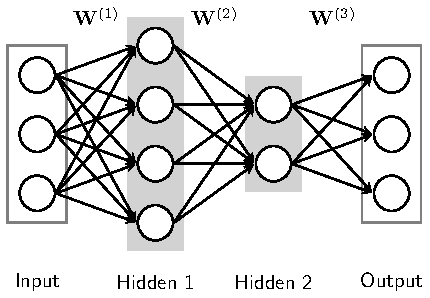
\includegraphics[width=.5\textwidth]{Chapters/05_NeuralNetworks/14_mlp/latex/multi_layers.pdf}
    }
\end{figure}

 
Số lượng tầng trong một mạng neuron đa tầng, được ký hiệu là $L$, được
tính bằng số tầng ẩn cộng với một. Khi đếm số tầng của một
mạng neuron đa tầng, ta không tính tầng đầu vào. Trong Hình~\ref{fig:14_3}, $L = 3$.
 
\subsection{Nút}
\index{nút -- node, unit}
Quan sát Hình~\ref{fig:14_4}, mỗi điểm hình tròn trong một tầng được
gọi là một \textit{nút} (node hoặc unit). Đầu vào của tầng ẩn thứ $l$ được ký hiệu bởi $\bz^{(l)}$, đầu ra tại mỗi tầng thường được ký
hiệu là $\ba^{(l)}$ (thể hiện \textit{activation}, tức giá trị tại các nút sau
khi áp dụng hàm kích hoạt lên đầu vào $\bz^{(l)}$). Đầu ra của nút
thứ $i$ trong tầng thứ $l$ được ký hiệu là $a_i^{(l)}$. Giả sử thêm rằng số
nút trong tầng thứ $l$ (không tính hệ số điều chỉnh) là $d^{(l)}$. Vector biểu diễn đầu ra
của tầng thứ $l$ là $\mathbf{a}^{(l)} \in \mathbb{R}^{d^{(l)}}$.
 
% \textit{Khi làm việc với những Neural Networks phức tạp, cách tốt nhất để hạn chế lỗi là viết cụ thể chiều của mỗi ma trận hay vector ra, bạn sẽ thấy rõ hơn trong phần sau.} 
 
 
\begin{figure}[t]
    % caption on side     
    \floatbox[{\capbeside\thisfloatsetup{capbesideposition={right,top},capbesidewidth=5cm}}]{figure}[\FBwidth]
    {\caption{ 
    Các ký hiệu sử dụng trong mạng neuron đa tầng.
    }
    \label{fig:14_4}}
    { % figure here
    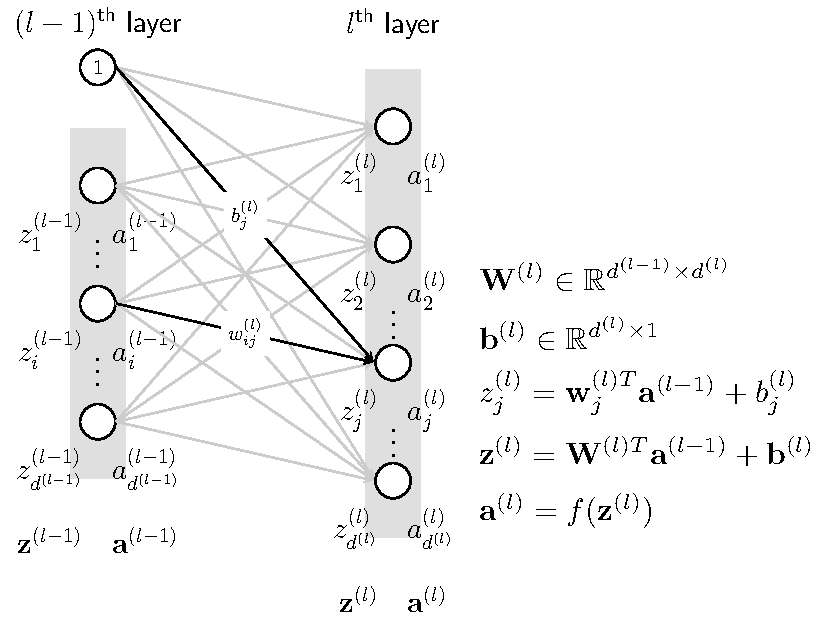
\includegraphics[width=.6\textwidth]{Chapters/05_NeuralNetworks/14_mlp/latex/mlp_notation.pdf}
    }
\end{figure}

 
\subsection{Trọng số và hệ số điều chỉnh}
Có $L$ ma trận trọng số cho một mạng neuron có $L$ tầng. Các ma
trận này được ký hiệu là $\mathbf{W}^{(l)} \in \mathbb{R}^{d^{(l-1)}\times
d^{(l)}}, l = 1, 2, \dots, L$ trong đó $\mathbf{W}^{(l)}$ thể hiện các
{kết nối} từ tầng thứ $l-1$ tới tầng thứ $l$ (nếu ta coi tầng đầu vào là
tầng thứ $0$). Cụ thể hơn, phần tử $w^{(l)}_{ij}$ thể hiện kết nối từ nút thứ
$i$ của tầng thứ $(l-1)$ tới nút từ $j$ của tầng thứ $(l)$. Các hệ số điều chỉnh của
tầng thứ $(l)$ được ký hiệu là $\mathbf{b}^{(l)} \in \mathbb{R}^{d^{(l)}}$. Các
trọng số này được ký hiệu trên Hình \ref{fig:14_4}. Khi tối ưu một
mạng neuron đa tầng cho một công việc nào đó, chúng ta cần đi tìm các
trọng số và hệ số điều chỉnh này. Tập hợp các trọng số và hệ số điều chỉnh lần lượt được ký hiệu là
$\mathbf{W}$ và $\mathbf{b}$. 
 
 
\section{Hàm kích hoạt}
\index{hàm kích hoạt -- activation function}

 
Mỗi đầu ra tại một tầng, trừ tầng đầu vào, được tính theo công thức:
\begin{equation} 
\ba^{(l)} = f^{(l)}(\mathbf{W}^{(l)T}\mathbf{a}^{(l-1)} + \bb^{(l)}).
\end{equation} 
 Trong đó $f^{(l)}(.)$ là một hàm kích hoạt phi tuyến. Nếu hàm kích hoạt tại một
tầng là một hàm tuyến tính, tầng này và tầng tiếp theo có thể rút gọn thành
một tầng vì {hợp của các hàm tuyến tính là một hàm tuyến tính}.

% \index{element-wise}
Hàm kích hoạt thường là một hàm số áp dụng lên {từng phần tử} của ma trận
hoặc vector đầu vào\footnote{Hàm softmax không áp dụng lên từng phần tử vì nó sử dụng mọi thành phần của vector đầu vào.}.

% Khi activation function $f(.)$ được áp dụng cho một ma trận (hoặc vector), ta hiểu rằng nó được áp dụng cho \textit{từng thành phần của ma trận đó}. Sau đó các thành phần này được sắp xếp lại đúng theo thứ tự để được một ma trận có kích thước bằng với ma trận input. 
 
 
\subsection{Hàm $\sgn$ không được sử dụng trong MLP}
 
\index{hàm kích hoạt -- activation function!sigmoid}
\index{hàm kích hoạt -- activation function!tanh}
Hàm $\sgn$ chỉ được sử dụng trong perceptron. Trong thực tế, hàm
$\sgn$ không được sử dụng vì đạo hàm tại hầu hết các điểm bằng không (trừ
tại gốc toạ độ không có đạo hàm). Việc đạo hàm bằng không này khiến cho các thuật toán dựa trên gradient không hoạt động.
 
\subsection{Sigmoid và tanh}
% \index{hàm kích hoạt -- activation function!sigmoid}
% \index{hàm kích hoạt -- activation function!tanh}
\begin{figure}[t]
    \begin{subfigure}{0.49\textwidth}
    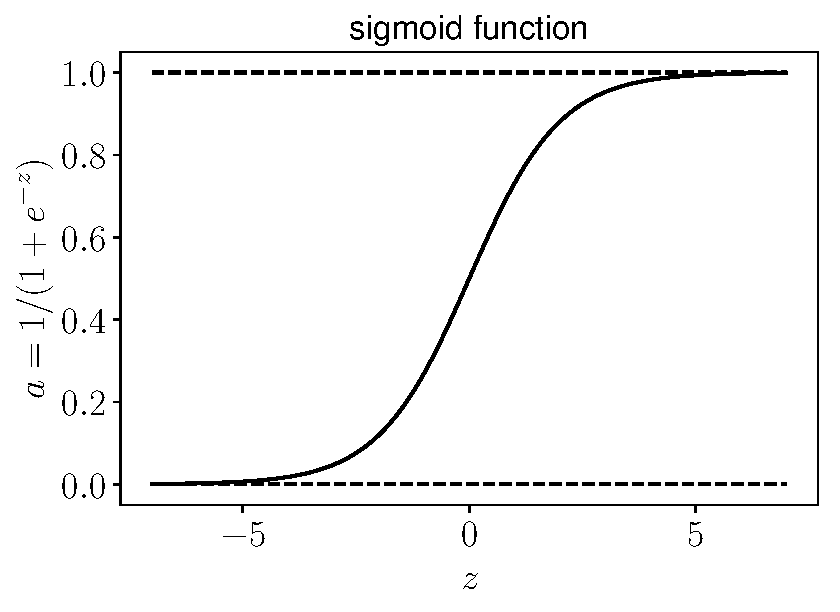
\includegraphics[width=0.99\linewidth]{ebookML_src/src/mlp/sigmoid.pdf}
    \caption{}
    \label{fig:14_5a}
    \end{subfigure}
    \begin{subfigure}{0.49\textwidth}
    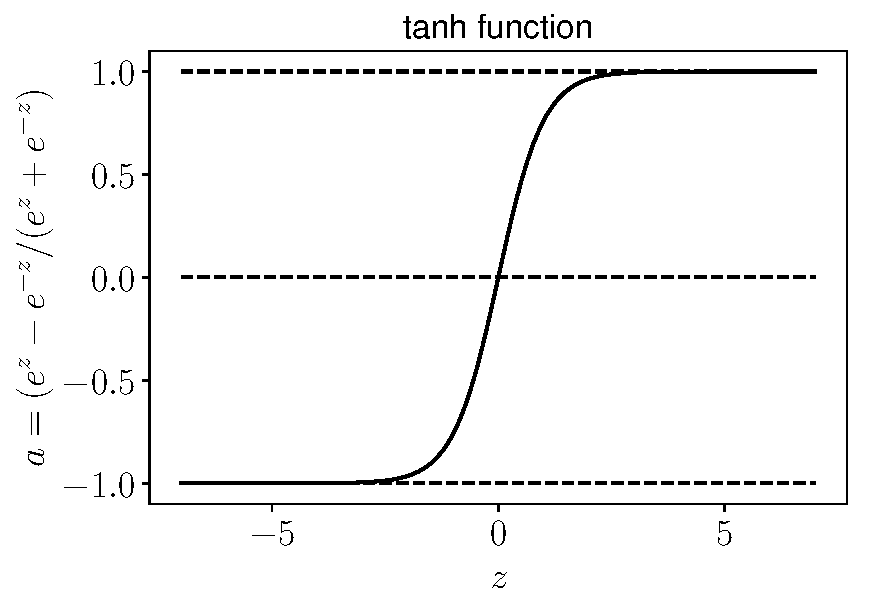
\includegraphics[width=0.99\linewidth]{ebookML_src/src/mlp/tanh.pdf}
    \caption{}
    \label{fig:14_5b}
    \end{subfigure}
    \caption{
     Ví dụ về đồ thị của hàm (a){sigmoid} và (b){tanh}.
    }
    \label{fig:14_5}
\end{figure}
%% *****************************************************************************
% \begin{figure}[t]
% \centering
%     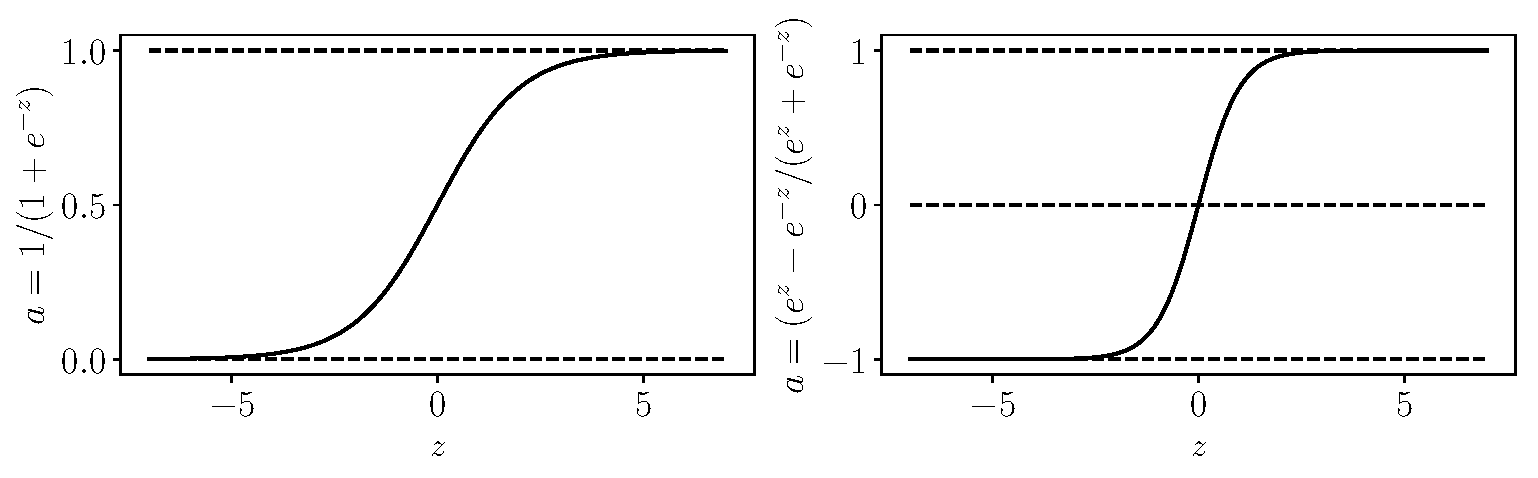
\includegraphics[width = \textwidth]{ebookML_src/src/mlp/sigmoid_tanh.pdf}
%     \caption[]{Đồ thị của hàm sigmoid và hàm tanh.}
%     \label{fig:14_5}
% \end{figure}
%% *****************************************************************************


 
Hàm sigmoid có dạng $\text{sigmoid}(z) = 1/(1 + \exp(-z))$ với đồ thị như
trong
Hình~\ref{fig:14_5a}. Nếu đầu vào lớn, hàm số sẽ cho đầu ra gần với một. Với đầu
vào nhỏ (rất âm), hàm số sẽ cho đầu ra gần với không. Trước đây, hàm kích hoạt này
được sử dụng nhiều vì có đạo hàm rất đẹp. Những năm gần đây, hàm số
này ít khi được sử dụng. Một hàm tương tự thường được sử dụng và mang lại hiệu
quả tốt hơn là hàm $\text{tanh}$ với $\displaystyle \text{tanh}(z) =
\frac{\exp(z) -
\exp{(-z)}}{\exp(z) + \exp(-z)}$. Hàm số
này có tính chất đầu ra chạy từ -1 đến 1, khiến cho nó có tính chất \textit{tâm không} (zero-centered) thay vì chỉ dương như hàm $\text{sigmoid}$. Gần đây, hàm sigmoid
chỉ được sử dụng ở tầng đầu ra khi đầu ra là các giá trị nhị phân hoặc biểu diễn các xác suất.
Một nhược điểm dễ nhận thấy là khi đầu vào có trị tuyệt đối lớn, đạo hàm của cả sigmoid và tanh rất gần với không. Điều này đồng nghĩa với
việc các hệ số tương ứng với nút đang xét sẽ gần như không được cập nhật khi sử
dụng công thức cập nhật gradient desent. Thêm nữa, khi khởi tạo các hệ số cho
mạng neuron đa tầng với hàm kích hoạt sigmoid, chúng cần tránh trường
hợp đầu vào một tầng ẩn nào đó quá lớn, vì khi đó đầu ra của tầng đó rất gần không hoặc một, dẫn đến đạo hàm bằng không và gradient desent hoạt động
không hiệu quả.


 
 
\subsection{ReLU}
 
\index{hàm kích hoạt -- activation function!ReLU}
% \index{ReLU!}
\begin{figure}[t]
    \begin{subfigure}{0.49\textwidth}
    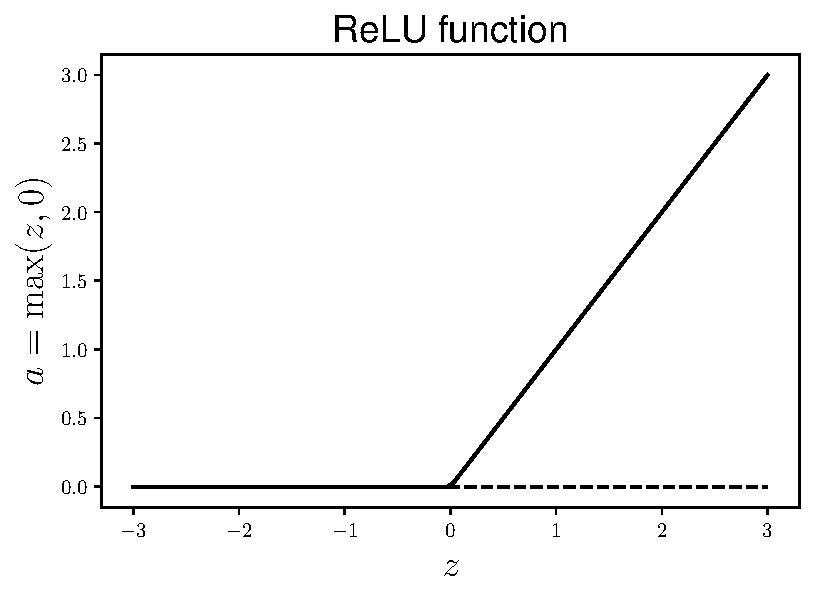
\includegraphics[width=0.99\linewidth]{ebookML_src/src/mlp/relu.pdf}
    \caption{}
    \label{fig:14_6a}
    \end{subfigure}
    \begin{subfigure}{0.49\textwidth}
    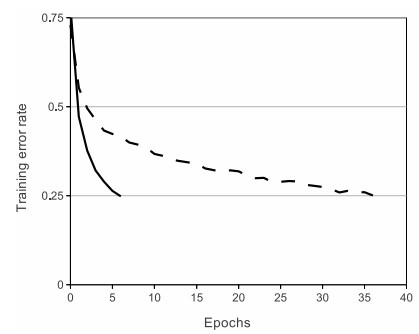
\includegraphics[width=0.99\linewidth]{Chapters/05_NeuralNetworks/14_mlp/alexplot.jpeg}
    \caption{}
    \label{fig:14_6b}
    \end{subfigure}
    \caption{
     Hàm ReLU và tốc độ hội tụ khi so sánh với hàm tanh.
    }
    \label{fig:14_6}
\end{figure}

ReLU (Rectified Linear Unit) gần đây được sử dụng rộng rãi vì tính đơn giản của
nó. Đồ thị của hàm ReLU được minh họa trên Hình~\ref{fig:14_6a}. Hàm ReLU có
công thức toán học $f(z) = \max(0, z)$ -- rất đơn giản trong tính toán.
Đạo hàm của nó bằng không tại các điểm âm, bằng một tại các điểm dương. ReLU được
chứng minh giúp việc huấn luyện các mạng neuron đa tầng nhanh hơn rất nhiều so với hàm
tanh~\cite{krizhevsky2012imagenet}. Hình~\ref{fig:14_6b} so sánh sự hội tụ của
hàm mất mát khi sử dụng hai hàm kích ReLU hoặc tanh. Ta thấy rằng với các mạng sử dụng hàm kích hoạt ReLU, hàm mất mát giảm rất nhanh sau một vài epoch đầu tiên. 

% Tại 0, đạo hàm của nó không
% xác định nhưng trên thực tế, có thể coi đạo hàm tại 0 bằng 0 hoặc 1. 

%  Ưu điểm chính của hàm ReLU là:
% \begin{itemize}
%     \item Mặc dù hàm ReLU không có đạo hàm tại $s = 0$, trong thực nghiệm, người
%     ta vẫn thường định nghĩa $\text{ReLU}'(0) = 0$ và khẳng định thêm rằng, xác
%     suất để input của một unit bằng 0 là rất nhỏ.

%     \item ReLU được chứng minh giúp cho việc huấn luyện các multilayer neural
%     network và deep network (rất nhiều hidden layer) nhanh hơn rất nhiều so với
%     hàm tanh~\cite{krizhevsky2012imagenet}. Hình~\ref{fig:14_6b} so sánh sự hội
%     tụ của hàm mất mát khi sử dụng hai hàm kích hoặc ReLU và tanh. Sự tăng tốc
%     này được cho là vì ReLU được tính toán gần như tức thời và gradient của nó
%     cũng được tính cực nhanh.
 
% \end{itemize}

Mặc dù cũng có nhược điểm đạo hàm bằng 0 với các giá trị đầu vào âm, ReLU được
chứng minh bằng thực nghiệm rằng có thể khắc phục việc này bằng việc tăng số
nút ẩn\footnote{\textit{Neural Networks and Deep Learning  --  Activation
function} (\url{https://goo.gl/QGjKmU}).}. Khi xây dựng một mạng neuron đa tầng, hàm kích hoạt ReLU nên được thử đầu tiên vì nó nhanh cho kết quả và thường hiệu quả trong nhiều trường hợp. Hầu hết các mạng neuron sâu 
đều có hàm kích hoạt là ReLU trong các tầng ẩn, trừ hàm kích hoạt ở tầng đầu ra vì nó phụ thuộc vào từng bài toán. 

Ngoài ra, các biến thể của ReLU như \textit{leaky rectified linear unit} (Leaky
ReLU), \textit{parametric rectified linear unit} (PReLU) và \textit{randomized
leaky rectified linear units} (RReLU)~\cite{xu2015empirical} cũng được sử dụng
và cho kết quả tốt. 



% \subsubsection{Một vài lưu ý}
% \begin{itemize}
% \item Output layer nhiều khi không có activation function mà sử dụng trực tiếp giá trị đầu vào $z_i^{(l)}$ của mỗi unit. Hoặc nói một cách khác, activation function chính là hàm \textit{identity}, tức đầu ra bằng đầu vào. Với các bài toán classification, output layer thường là một \href{http://machinelearningcoban.com/2017/02/17/softmax/}{Softmax Regression} layer giúp tính xác suất để một điểm dữ liệu rơi vào mỗi class. 
 
% \item Mặc dù activation function cho mỗi unit có thể khác nhau, trong cùng một network, activation như nhau thường được sử dụng. Điều này giúp cho việc tính toán được đơn giản hơn. 
% \end{itemize}
 

 
\section{Lan truyền ngược}
\index{lan truyền ngược -- backpropagation}

Phương pháp phổ biến nhất để tối ưu mạng neuron đa tầng chính là gradient
descent (GD). Để áp dụng GD, chúng ta cần tính được gradient của hàm mất mát
theo từng ma trận trọng số $\mathbf{W}^{(l)}$ và vector điều chỉnh $\mathbf{b}^{(l)}$.

% \end{equation} 
 
% Bước này được gói là \textit{feedforward} vì cách tính toán được thực hiện từ đầu đến cuối của network. MLP cũng được gọi 
 
Giả sử $J(\mathbf{W, b, X, Y})$ là một hàm mất mát của bài toán, trong đó
$\mathbf{W, b}$ là tập hợp tất cả các ma trận trọng số và vector điều chỉnh. $\mathbf{X, Y}$ là cặp dữ liệu huấn luyện với mỗi cột
tương ứng với một điểm dữ liệu. Để có thể áp dụng các phương pháp gradient descent,
chúng ta cần tính được các 
% \begin{equation} 
% \frac{\partial J}{\partial \mathbf{W}^{(l)}} ; \frac{\partial J}{\partial \mathbf{b}^{(l)}},~~ l = 1, 2, \dots, L 
% \end{equation} 
\begin{math}
    \nabla_{\bW^{(l)}}J; \nabla_{\bb^{(l)}}J, ~\forall l = 1, 2, \dots, L
\end{math}.

Nhắc lại quá trình lan truyền thuận: 
\begin{eqnarray} 
\mathbf{a}^{(0)} &=& \mathbf{x} \\\
\mathbf{z}^{(l)}  &=& \mathbf{W}^{(l)T}\mathbf{a}^{(l-1)} + \mathbf{b}^{(l)},~~ l =  1, 2, \dots, L \\\ 
\mathbf{a}^{(l)} &=& f^{(l)}(\mathbf{z}^{(l)}), ~~ l =  1, 2, \dots, L \\\ 
\mathbf{\hat{y}} &=& \mathbf{a}^{(L)} 
\end{eqnarray} 

\index{sai số trung bình bình phương -- MSE}

Xét ví dụ của hàm mất mát là hàm sai số trung bình bình phương (MSE):
 % tức \textit{trung bình của bình phương lỗi} trong bài toán regression
\begin{eqnarray} 
J(\mathbf{W, b, X, Y}) &=& \frac{1}{N}\sum_{n=1}^N \| \mathbf{y}_n - \mathbf{\hat{y}}_n\|_2^2 
=\frac{1}{N}\sum_{n=1}^N \| \mathbf{y}_n - \mathbf{a}_n^{(L)}\|_2^2 
\end{eqnarray} 
với $N$ là số cặp dữ liệu $(\mathbf{x}, \mathbf{y})$ trong tập huấn luyện. Theo
các công thức này, việc tính toán trực tiếp các giá trị gradient tương đối phức
tạp vì hàm mất mát không phụ thuộc trực tiếp vào các ma trận trọng số và vector
điều chỉnh. Phương pháp phổ biến nhất được dùng có tên là \textit{lan truyền ngược}
(backpropagation) giúp tính gradient ngược từ tầng cuối cùng đến tầng đầu tiên.
Tầng cuối cùng được tính toán trước vì nó ảnh hưởng trực tiếp tới {đầu ra dự
đoán} và hàm mất mát. Việc tính toán gradient của các ma trận trọng số trong các
tầng trước được thực hiện dựa trên quy tắc chuỗi quen thuộc cho {gradient của hàm
hợp}.
 
Stochastic gradient descent có thể được sử dụng để cập nhật các ma trận trọng số và vector điều chỉnh dựa trên một cặp điểm huấn luyện $\mathbf{x, y}$. Đơn giản hơn, ta coi $J$ là hàm mất mát nếu chỉ xét cặp điểm này. Ở đây $J$ là hàm mất mát bất kỳ, không chỉ hàm MSE như ở trên. 
 Đạo hàm riêng của hàm mất mát theo \textit{chỉ một thành phần} của ma trận trọng số
của tầng đầu ra:
\begin{eqnarray} 
\frac{\partial J}{\partial w_{ij}^{(L)}} &=& \frac{\partial J}{\partial
z_j^{(L)}}. \frac{\partial z_j^{(L)}}{\partial w_{ij}^{(L)}} = e_j^{(L)} a_i^{(L-1)} 
\end{eqnarray} 
trong đó $\displaystyle e_j^{(L)} = \frac{\partial J}{\partial z_j^{(L)}} $
thường là một đại
lượng {không quá khó để tính toán} và $\displaystyle\frac{\partial
z_j^{(L)}}{\partial w_{ij}^{(L)}}  = a_i^{(L-1)}$ vì $z_j^{(L)} = \mathbf{w}_j^{(L)T}\mathbf{a}^{(L-1)} + b_j^{(L)}$.
Tương tự, gradient của hàm mất mát theo hệ số tự do của tầng cuối cùng là
\begin{equation} 
\frac{\partial J}{\partial b_{j}^{(L)}} = \frac{\partial J}{\partial z_j^{(L)}}. \frac{\partial z_j^{(L)}}{\partial b_{j}^{(L)}} = e_j^{(L)} 
\end{equation} 
Với đạo hàm riêng theo trọng số ở các tầng $l < L$, hãy quan sát Hình
\ref{fig:14_6_2}. Ở đây, tại mỗi nút, đầu vào $z$ và đầu ra $a$ được viết
riêng để tiện theo dõi.

Dựa vào Hình \ref{fig:14_6_2}, bằng quy nạp ngược từ cuối, ta có thể tính được:
\begin{eqnarray} 
\frac{\partial J}{\partial w_{ij}^{(l)}} &=& \frac{\partial J}{\partial
z_j^{(l)}}. \frac{\partial z_j^{(l)}}{\partial w_{ij}^{(l)}} = e_j^{(l)} a_i^{(l-1)}. 
\end{eqnarray} 
\newpage
với:
\begin{eqnarray*} 
e_j^{(l)} &=& \frac{\partial J}{\partial z_j^{(l)}} = \frac{\partial J}{\partial a_j^{(l)}} . \frac{\partial a_j^{(l)}}{\partial z_j^{(l)}} \\\ 
&=& \left( \sum_{k = 1}^{d^{(l+1)}} \frac{\partial J}{\partial z_k^{(l+1)}}
.\frac{\partial z_k^{(l+1)}}{\partial a_j^{(l)}} \right) f^{(l)'}(z_j^{(l)}) =\left( \sum_{k = 1}^{d^{(l+1)}} e_k^{(l+1)} w_{jk}^{(l+1)} \right)
 f^{(l)'}(z_j^{(l)}) \\
 &=& \left(\bw_{j:}^{(l+1)}\be^{(l+1)}f^{(l)'}\right)(z_j^{(l)})
\end{eqnarray*} 
trong đó $\mathbf{e}^{(l+1)} = [e_1^{(l+1)}, e_2^{(l+1)}, ...,
e_{d^{(l+1)}}^{(l+1)}]^T \in \mathbb{R}^{d^{(l+1)}\times 1} $ và
$\mathbf{w}_{j:}^{(l+1)}$ được hiểu là \textbf{hàng} thứ $j$ của ma trận
$\mathbf{W}^{(l+1)}$ (chú ý dấu hai chấm, khi không có dấu này, chúng ta mặc
định dùng nó để ký hiệu cho vector \textit{cột}).
 Dấu $\sum$ tính tổng ở dòng thứ hai trong phép tính trên xuất hiện vì
$a_{j}^{(l)}$ {đóng góp} vào việc tính tất cả các $z_k^{(l+1)}, k = 1, 2,
\dots, d^{(l+1)}$. Biểu thức đạo hàm ngoài dấu ngoặc lớn xuất hiện vì $a_j^{(l)}  =
f^{(l)}(z_j^{(l)})$. Tới đây, ta có thể thấy rằng việc hàm kích hoạt có
đạo hàm đơn giản sẽ có ích rất nhiều trong việc tính toán.
\begin{figure}[t]
\centering
    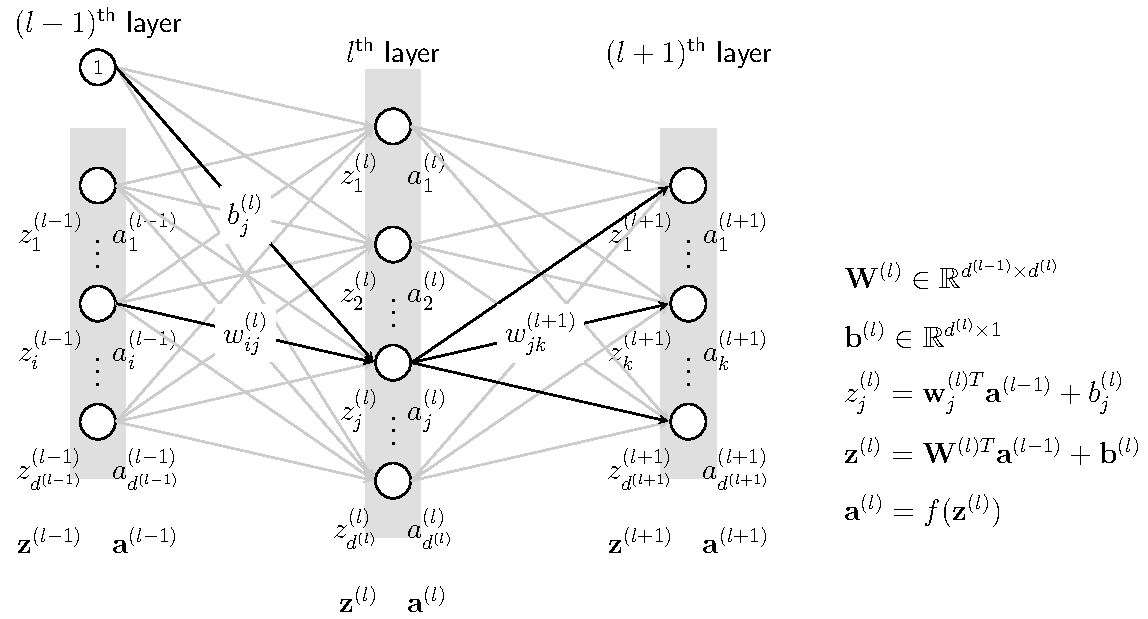
\includegraphics[width =
    .95\textwidth]{Chapters/05_NeuralNetworks/14_mlp/latex/backpropagation.pdf}
    \caption[]{Mô phỏng cách tính lan truyền ngược. Tầng cuối có thể là tầng đầu ra.}
    \label{fig:14_6_2}
\end{figure}
Với cách làm tương tự, bạn đọc có thể suy ra
\begin{equation} 
\frac{\partial J}{\partial b_j^{(l)}} = e_j^{(l)}.
\end{equation}
Nhận thấy rằng trong những công thức trên, việc tính các $e_j^{(l)}$ đóng một vài trò quan trọng. Hơn nữa, để tính được giá trị này, ta cần tính được các $e_j^{(l+1)}$. Nói cách khác, ta cần tính {ngược} các giá trị này từ tầng cuối cùng. tên gọi \textit{lan truyền ngược} xuất phát từ đây.
 
Tóm tắt quá trình tính toán gradient cho ma trận trọng số và vector điều chỉnh tại mỗi tầng:
 
 
% \subsection{Backpropagation cho Stochastic Gradient Descent}
 
 
% \textbf{Đạo hàm theo từng hệ số} $w_{ij}^{(l)}, b_{i}^{(l)}$
\begin{myalg}{{Lan truyền ngược tới} $w_{ij}^{(l)},
b_{i}^{(l)}$}{label0}
\begin{enumerate}
    \item[1.] Lan truyền thuận: Với 1 giá trị đầu vào $\mathbf{x}$, tính giá trị đầu
    ra của mạng, trong quá trình tính toán, lưu lại các giá trị $\mathbf{a}^{(l)}$ tại mỗi tầng.
    \item[2.] Với mỗi nút $j$ ở tầng đầu ra, tính:
    % \begin{equation}
    % \end{equation}
    % \item  Từ đó suy ra:
    \begin{eqnarray} 
    e_j^{(L)} = \frac{\partial J}{\partial z_j^{(L)}}; \quad 
    \frac{\partial J}{\partial w_{ij}^{(L)}} = a_i^{(L-1)}e_j^{(L)}; \quad  
    \frac{\partial J}{\partial b_{j}^{(L)}} = e_j^{(L)} 
    \end{eqnarray} 

    \item[3.]  Với $l = L-1, L-2, ..., 1$, tính: 
    \begin{equation} 
    e_j^{(l)} = \left( \mathbf{w}_{j:}^{(l+1)} \mathbf{e}^{(l+1)} \right) f'(z_j^{(l)}) 
    \end{equation} 

    \item[4.] Cập nhật gradient cho từng thành phần:
    \begin{eqnarray} 
    \frac{\partial J}{\partial w_{ij}^{(l)}} = a_i^{(l-1)} e_j^{(l)}; \quad 
    \frac{\partial J}{\partial b_{j}^{(l)}} = e_j^{(l)} 
    \end{eqnarray} 
\end{enumerate}
\end{myalg}
 
 
 
Phiên bản vector hoá của thuật toán trên có thể được thực hiện như
sau:
% \subsubsection{Đạo hàm theo ma trận $\mathbf{W}^{(l)}, \mathbf{b}^{(l)}$}
% Việc tính toán theo từng hệ số như trên chỉ phù hợp cho việc hiểu nguyên lý tính toán, trong khi lập trình, ta cần tìm cách thu gọn chúng về dạng vector và ma trận để tăng tốc độ cho thuật toán. Đặt $\mathbf{e}^{(l)} = [e_1^{(l)}, e_2^{(l)}, ..., e_{d^{(l)}}^{(l)}]^T \in \mathbb{R}^{d^{(l)}\times 1} $. Ta sẽ có quy tắc tính như sau: 
\index{tích từng thành  phân -- Hadamard product}
% ******************************************************************************
\begin{myalg}{Lan truyền ngược tới $\bW^{(l)}$ và $\bb^{(l)}$}{label}
\begin{enumerate}
    \item[1.] Lan truyền thuận: Với một giá trị đầu vào $\mathbf{x}$, tính giá trị đầu
    ra của mạng, trong quá trình tính toán, lưu lại các $\mathbf{a}^{(l)}$ tại mỗi tầng.

    \item[2.] Với tầng đầu ra, tính:
    % \begin{equation}
    % \item Từ đó suy ra: 
    %     \end{equation} 
    % \begin{eqnarray*} 
    %     \mathbf{e}^{(L)} = \frac{\partial J}{\partial \mathbf{z}^{(L)}} \in 
    %     \R^{d^{(L)}};~
    %     \frac{\partial J}{\partial \mathbf{W}^{(L)}} =
    %     \mathbf{a}^{(L-1)}\mathbf{e}^{(L)T} \in \R^{d^{(L-1)}\times d^{(L)}};
    %     ~
    %     \frac{\partial J}{\partial \mathbf{b}^{(L)}} =  \mathbf{e}^{(L)}
    % \end{eqnarray*} 
    \begin{eqnarray*} 
        \mathbf{e}^{(L)} = \nabla_{\bz^{(L)}}J \in
        \R^{d^{(L)}};~
        \nabla_{\mathbf{W}^{(L)}}J =
        \mathbf{a}^{(L-1)}\mathbf{e}^{(L)T} \in \R^{d^{(L-1)}\times d^{(L)}};
        ~
        \nabla_{\mathbf{b}^{(L)}}J =  \mathbf{e}^{(L)}
    \end{eqnarray*} 
    \item[3.] Với $l = L-1, L-2, ..., 1$, tính: 
    \begin{equation} 
    \mathbf{e}^{(l)} = \left( \mathbf{W}^{(l+1)} \mathbf{e}^{(l+1)} \right)
    \odot f'(\mathbf{z}^{(l)}) \in \R^{d^{(l)}}
    \end{equation} 
    trong đó $\odot$ là tích \textit{Hadamard}, tức lấy từng thành phần của hai vector nhân với nhau để được vector kết quả. 
    \item[4.] Cập nhật gradient cho các ma trận trọng số và vector điều chỉnh: 
    \begin{eqnarray} 
    \nabla_{\mathbf{W}^{(l)}}J =
    \mathbf{a}^{(l-1)}\mathbf{e}^{(l)T} \in \R^{d^{(l-1)}\times d^{(l)}}; \quad 
    \nabla_{\mathbf{b}^{(l)}}J = \mathbf{e}^{(l)} 
\end{eqnarray} 
 \end{enumerate} 
\end{myalg}
% ******************************************************************************
 
Khi làm việc với các phép tính gradient phức tạp, ta luôn cần nhớ hai điều sau:
\begin{itemize}
    \item Gradient của một hàm có đầu ra là một số vô hướng theo một vector hoặc
    ma trận là một đại lượng có cùng chiều với vector hoặc ma trận đó. 

    \item Phép nhân ma trận và vector thực hiện được chỉ khi chúng có chiều phù hợp.
\end{itemize}
 
Trong công thức $ \nabla_{\mathbf{W}^{(L)}}J =
\mathbf{a}^{(L-1)}\mathbf{e}^{(L)T}$, vế trái là một ma trận thuộc
$\R^{d^{(L-1)}\times d^{(L)}}$, vậy vế phải cũng phải là một đại lượng có chiều
tương tự. Từ đó bạn đọc có thể thấy tại sao vế phải phải là
$\mathbf{a}^{(L-1)}\mathbf{e}^{(L)T}$ mà không thể là
$\mathbf{a}^{(L-1)}\mathbf{e}^{(L)}$ hay $\mathbf{e}^{(L)}\mathbf{a}^{(L-1)}$.



% \textbf{Chú ý:} Biểu thức tính đạo hàm trong dòng trên của bước 3 có thể khiến bạn đặt câu hỏi: tại sao lại là $\mathbf{a}^{(L-1)}\mathbf{e}^{(L)T}$ mà không phải là $\mathbf{a}^{(L-1)T}\mathbf{e}^{(L)}$, $\mathbf{e}^{(L)T}\mathbf{a}^{(L-1)}$, hay $\mathbf{e}^{(L)}\mathbf{a}^{(L-1)T}$? \textit{Quy tắc bỏ túi} cần nhớ là \textbf{chiều của hai ma trận ở hai vế phải như nhau}. Thử một chút, vế trái là đạo hàm theo $\mathbf{W}^{(L)}$ là một đại lượng có chiều (\textit{dimension}, not \textit{afternoon}) bằng chiều của ma trận này, tức chiều là $\mathbb{R}^{d^{(L-1)}\times d^{(L)}}$. Vế phải, $\mathbf{e}^{(L)} \in \mathbf{R}^{d^{(L)} \times 1}$, $\mathbf{a}^{(L-1)} \in \mathbb{R}^{d^{(L-1)} \times 1}$. Để hai vế có chiều bằng nhau thì ta phải lấy $\mathbf{a}^{(L-1)} \mathbf{e}^{(L)T}$. Cũng chú ý thêm \textbf{rằng đạo hàm theo một ma trận của một hàm số nhận giá trị thực (scalar) sẽ có chiều bằng với chiều của ma trận đó!!} 
 
 
\subsection{Lan truyền ngược cho một mini-batch}
 
Nếu ta muốn thực hiện batch hoặc mini-batch GD thì thế nào? Trong thực tế,
mini-batch GD được sử dụng nhiều nhất với các bài toán mà tập huấn luyện lớn.
Nếu lượng dữ liệu nhỏ, batch GD trực tiếp được sử dụng. Khi đó, cặp (đầu vào,
đầu ra) sẽ ở dạng ma trận $(\mathbf{X, Y})$. Giả sử
 mỗi mini-batch có $N$ dữ liệu. Khi đó, $\mathbf{X} \in \mathbb{R}^{d^{(0)} \times N}, \mathbf{Y} \in \mathbb{R}^{d^{(L)}\times N}$. Với $d^{(0)} = d$ là chiều của dữ liệu đầu vào. 
 
Khi đó các activation sau mỗi layer sẽ có dạng $\mathbf{A}^{(l)} \in \mathbb{R}^{d^{(l)} \times N}$. Tương tự, $\mathbf{E}^{(l)} \in \mathbb{R}^{d^{(l)}\times N}$. Và ta cũng có thể suy ra công thức cập nhật như sau:

% \index{Hadamard product}
% ******************************************************************************
 \begin{myalg}{Lan truyền ngược tới $\bW^{(l)}$ và $\bb^{(l)}$ (mini-batch)}{backprop_batch}
\begin{enumerate}
 \item Lan truyền thuận: Với toàn bộ dữ liệu hoặc một mini-batch đầu vào
 $\mathbf{X}$, tính giá trị đầu ra của mạng, trong quá trình tính toán, lưu lại
 các $\mathbf{A}^{(l)}$ tại mỗi tầng. Mỗi cột của $\mathbf{A}^{(l)}$ tương ứng
 với một cột của $\mathbf{X}$, tức một điểm dữ liệu đầu vào.
 \item Tại tầng đầu ra, tính:
  % \begin{equation}
 % \item Từ đó suy ra: 
  % \end{equation} 
 % \begin{eqnarray} 
 %  \mathbf{E}^{(L)} = \frac{\partial J}{\partial \mathbf{Z}^{(L)}}; \quad 
 % \frac{\partial J}{\partial \mathbf{W}^{(L)}} = 
 % \mathbf{A}^{(L-1)}\mathbf{E}^{(L)T}; \quad
 % \frac{\partial J}{\partial \mathbf{b}^{(L)}} =  \sum_{n=1}^N\mathbf{e}_n^{(L)} 
 % \end{eqnarray} 
  \begin{eqnarray*} 
  \mathbf{E}^{(L)} = \nabla_{\mathbf{Z}^{(L)}}J; \quad 
 \nabla_{\mathbf{W}^{(L)}}J = 
 \mathbf{A}^{(L-1)}\mathbf{E}^{(L)T}; \quad
 \nabla_{\mathbf{b}^{(L)}}J =  \sum_{n=1}^N\mathbf{e}_n^{(L)} 
 \end{eqnarray*} 
 \item Với $l = L-1, L-2, ..., 1$, tính: 
 \begin{equation*} 
 \mathbf{E}^{(l)} = \left( \mathbf{W}^{(l+1)} \mathbf{E}^{(l+1)} \right) \odot f'(\mathbf{Z}^{(l)}) 
 \end{equation*} 

 \item Cập nhật gradient cho ma trận trọng số và vector điều chỉnh: 
 \begin{eqnarray*} 
 \nabla_{\mathbf{W}^{(l)}}J = 
 \mathbf{A}^{(l-1)}\mathbf{E}^{(l)T}; \quad 
 \nabla_{\mathbf{b}^{(l)}}J =  \sum_{n=1}^N\mathbf{e}_n^{(l)} 
 \end{eqnarray*} 
 \end{enumerate}
 \end{myalg}
% ******************************************************************************
 
 
 
 % Mặc dù khi làm thực nghiệm, các công cụ có hỗ trợ việc tự động tính Backpropagation, tôi vẫn không muốn bỏ qua phần này. Hiểu backpropagation rất quan trọng! Xem thêm \href{https://medium.com/@karpathy/yes-you-should-understand-backprop-e2f06eab496b#.g76s9xxzc}{Yes you should understand backprop}. 
 
 
\section{Ví dụ trên Python}
% Source code cho ví dụ này có thể được xem \href{https://github.com/tiepvupsu/tiepvupsu.github.io/blob/master/assets/14_mlp/Example%20.ipynb}{tại đây}. 
 
 

Trong mục này, chúng ta sẽ tạo dữ liệu giả trong không gian hai chiều sao cho
đường ranh giới giữa các class {không} có dạng tuyến tính. Điều này khiến hồi
quy softmax không làm việc được. Tuy nhiên, bằng cách thêm một tầng ẩn, chúng ta
sẽ thấy rằng mạng neuron này làm việc rất hiệu quả.
 
\subsection{Tạo dữ liệu giả}
 
% Trước hết, ta tạo dữ liệu cho 3 classes mà không có hai class nào là \textit{linearly separable}: 
 
% \begin{lstlisting}[language=Python]
% # To support both python 2 and python 3 
% from __future__ import division, print_function, unicode_literals 
% import math 
% import numpy as np 
% import matplotlib.pyplot as plt 
 
% N = 100 # number of points per class 
% d0 = 2 # dimensionality 
% C = 3 # number of classes 
% X = np.zeros((d0, N*C)) # data matrix (each row = single example) 
% y = np.zeros(N*C, dtype='uint8') # class labels 
 
% for j in xrange(C): 
%   ix = range(N*j,N*(j+1)) 
%   r = np.linspace(0.0,1,N) # radius 
%   t = np.linspace(j*4,(j+1)*4,N) + np.random.randn(N)*0.2 # theta 
%   X[:,ix] = np.c_[r*np.sin(t), r*np.cos(t)].T 
%   y[ix] = j 
% # lets visualize the data: 
% # plt.scatter(X[:N, 0], X[:N, 1], c=y[:N], s=40, cmap=plt.cm.Spectral) 
 
% plt.plot(X[0, :N], X[1, :N], 'bs', markersize = 7); 
% plt.plot(X[0, N:2*N], X[1, N:2*N], 'ro', markersize = 7); 
% plt.plot(X[0, 2*N:], X[1, 2*N:], 'g^', markersize = 7); 
% # plt.axis('off') 
% plt.xlim([-1.5, 1.5]) 
% plt.ylim([-1.5, 1.5]) 
% cur_axes = plt.gca() 
% cur_axes.axes.get_xaxis().set_ticks([]) 
% cur_axes.axes.get_yaxis().set_ticks([]) 
 
% plt.savefig('EX.png', bbox_inches='tight', dpi = 600) 
% plt.show() 
% \end{lstlisting}

Các điểm dữ liệu giả của ba lớp được tạo và minh hoạ bởi các điểm vuông, tròn,
tam giác trong Hình~\ref{fig:14_7a}. Ta thấy rõ ràng rằng đường ranh giới giữa
các lớp dữ liệu không thể là các đường thẳng. Hình~\ref{fig:14_7b} là một ví dụ
về các đường ranh giới được coi là tốt với hầu hết các điểm dữ liệu. Các đường
ranh giới này tạo được bởi một mạng neuron với một tầng ẩn sử dụng ReLU làm hàm
kích hoạt và tầng đầu ra là một hồi quy softmax như trong Hình~\ref{fig:14_8}.
Chúng ta cùng đi sâu vào xây dựng bộ phân loại dựa trên dữ liệu huấn luyện này.% \begin{figure}[t]Ta t 
%     % caption on side     
%     \floatbox[{\capbeside\thisfloatsetup{capbesideposition={right,top},capbesidewidth=6cm}}]{figure}[\FBwidth]
%     {\caption{ 
%     Phân bố dữ liệu của các lớp.
%     }
%     \label{fig:14_7}}
%     { % figure here
%     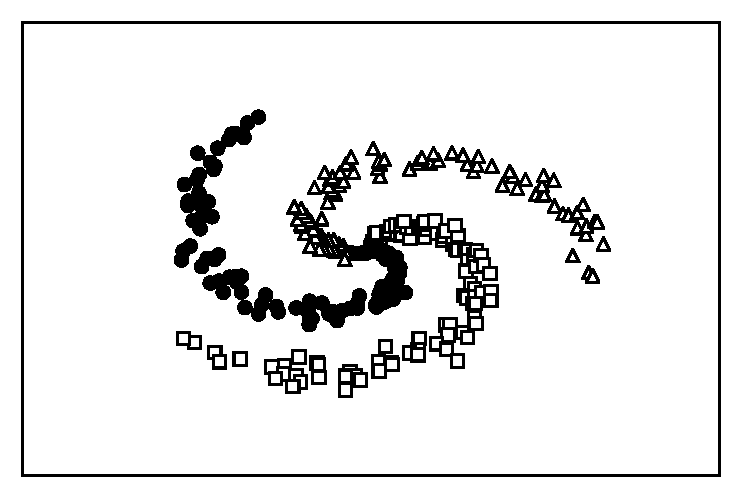
\includegraphics[width=.5\textwidth]{ebookML_src/src/mlp/EX.pdf}
%     }
% \end{figure}

%% *****************************************************************************
 \begin{figure}[t]
     \begin{subfigure}{0.45\textwidth}
     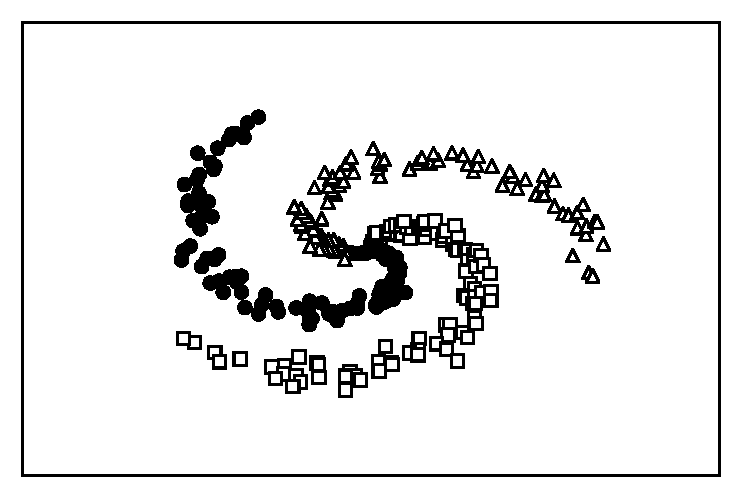
\includegraphics[width=0.99\linewidth]{ebookML_src/src/mlp/EX.pdf}
     \caption{}
     \label{fig:14_7a}
     \end{subfigure}
     \begin{subfigure}{0.45\textwidth}
     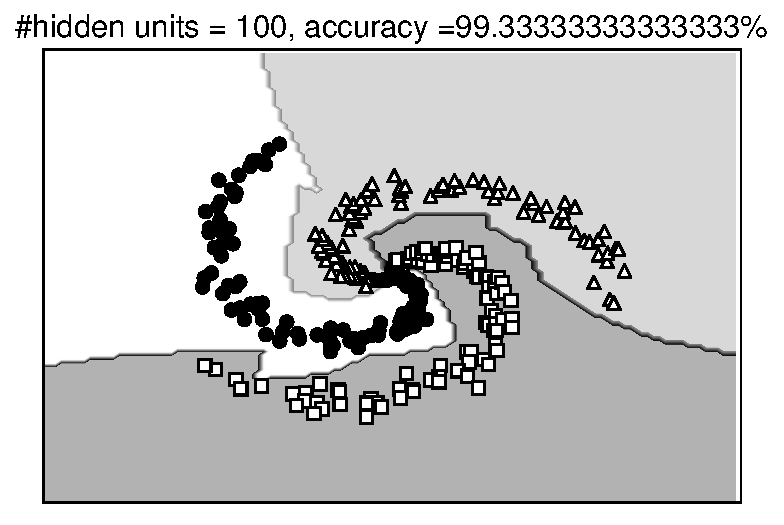
\includegraphics[width=0.99\linewidth]{ebookML_src/src/mlp/ex_res100.pdf}
     \caption{}
     \label{fig:14_7b}
     \end{subfigure}
     \caption{
     Dữ liệu giả trong không gian hai chiều và ví dụ về các ranh giới tốt.  
     }
     \label{fig:14_7}
 \end{figure}
 %% *****************************************************************************
  
% Với dữ liệu được phân bố thế này, Softmax Regression không thể thực hiện được vì \href{http://machinelearningcoban.com/2017/02/17/softmax/#-boundary-tao-boi-softmax-regression-la-linear}{Bounray giữa các class tạo bởi Softmax Regression có dạng linear}. Chúng ta hãy làm một thí nghiệm nhỏ bằng cách thêm một \textit{Hidden layer} vào giữa Input layer vả output layer của Softmax Regression. 

\begin{figure}[t]
    % caption on side     
    \floatbox[{\capbeside\thisfloatsetup{capbesideposition={right,top},capbesidewidth=6cm}}]{figure}[\FBwidth]
    {\caption{ 
    Mạng neuron đa tầng với tầng đầu vào có hai nút (nút điều chỉnh đã được ẩn),
    một tầng ẩn với hàm kích hoạt ReLU (có thể có số lượng nút ẩn
    tuỳ ý), và tầng đầu ra là một hồi quy softmax với ba phần tử đại diện
    cho ba lớp dữ liệu. 
    }
    \label{fig:14_8}}
    { % figure here
    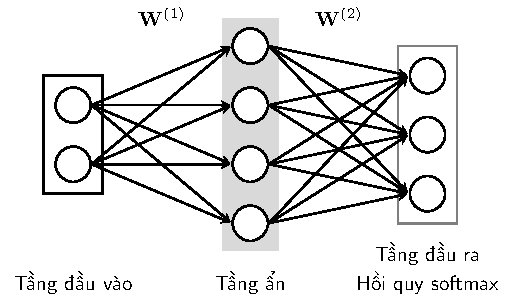
\includegraphics[width=.5\textwidth]{Chapters/05_NeuralNetworks/14_mlp/latex/ex_nn.pdf}
    }
\end{figure}
% \newpage 
Nhắc lại hàm ReLU $f(z) = \max(z, 0)$, với đạo hàm:
\begin{equation}
    f'(z) = \left\{ 
    \begin{matrix}
        0 & \text{nếu}~ z \leq 0 \\ 
        1 & \text{o.w}
    \end{matrix}
    \right. 
\end{equation}
Vì lượng dữ liệu huấn luyện nhỏ chỉ với 100 điểm cho mỗi lớp, ta có thể dùng
batch GD để cập nhật các ma trận trọng số và vector điều chỉnh. Trước hết, ta cần tính
gradient của hàm mất mát theo các ma trận và vector này bằng lan truyền ngược.

% Bây giờ chúng ta sẽ áp dụng Batch Gradient Descent cho bài toán này (vì lượng dữ liệu là nhỏ). Trước hết cần thực tìm công thức tính các activation và output. 
 
\subsection{Tính toán lan truyền thuận}
Giả sử các cặp dữ liệu huấn luyện là $(\bx_i, \by_i)$ với $\by_i$ là một vector
ở dạng one-hot. Các điểm dữ liệu này xếp cạnh nhau tạo thành các ma trận đầu
vào $\bX$ và ma trận đầu ra $\bY$. Bước lan truyền thuận được
thực hiện như sau:
\begin{eqnarray} 
\mathbf{Z}^{(1)} &=& \mathbf{W}^{(1)T}\mathbf{X} + \bB^{(1)}\\\ 
\mathbf{A}^{(1)} &=& \max(\mathbf{Z}^{(1)}, \mathbf{0}) \\\ 
\mathbf{Z}^{(2)} &=& \mathbf{W}^{(2)T}\mathbf{A}^{(1)} + \bB^{(2)}\\\ 
\mathbf{\hat{Y}} &=& \mathbf{A}^{(2)} = \text{softmax}(\mathbf{Z}^{(2)}) 
\end{eqnarray} 
Trong đó $\bB^{(1)}, \bB^{(2)}$ là các ma trận điều chỉnh với tất cả các cột bằng nhau
lần lượt bằng $\bb^{(1)}$ và $\bb^{(2)}$\footnote{Ta cần xếp các vector điều chỉnh
giống nhau để tạo thành các ma trận điều chỉnh vì trong toán học, không có định nghĩa
tổng của một ma trận và một vector. Khi lập trình, việc này là khả thi.}.
Hàm mất mát được sử dụng là hàm entropy chéo:
\begin{equation} 
J \triangleq J(\mathbf{W, b}; \mathbf{X, Y}) = -\frac{1}{N}\sum_{i = 1}^N \sum_{j = 1}^C y_{ji}\log(\hat{y}_{ji}) 
\end{equation} 
% Ở đây, tôi đã cho thêm thừa số $\frac{1}{N}$ để tránh hiện tượng tổng quá lớn với Batch GD. Về mặt toán học, thừa số này không làm thay đổi nghiệm của bài toán. 
 
 
\subsection{Tính toán lan truyền ngược}
Áp dụng Thuật toán~\ref{alg:backprop_batch}, ta có 
\begin{eqnarray} 
\mathbf{E}^{(2)} &=& \nabla_{\mathbf{Z}^{(2)}}
=\frac{1}{N}(\bA^{(2)}- \mathbf{Y}) \\\ 
\nabla_{\mathbf{W}^{(2)}} &=& \mathbf{A}^{(1)} 
\mathbf{E}^{(2)T}; \quad 
\nabla_{\mathbf{b}^{(2)}} = \sum_{n=1}^N\mathbf{e}_n^{(2)}
\\\ 
\mathbf{E}^{(1)} &=& \left(\mathbf{W}^{(2)}\mathbf{E}^{(2)}\right) \odot
f'(\mathbf{Z}^{(1)}) \\\
\nabla_{\mathbf{W}^{(1)}} &=& \mathbf{A}^{(0)} 
\mathbf{E}^{(1)T} = \mathbf{X}\mathbf{E}^{(1)T};\quad 
\nabla_{\mathbf{b}^{(1)}} = \sum_{n=1}^N\mathbf{e}_n^{(1)}
\end{eqnarray} 
Các công thức toán học phức tạp này sẽ được lập trình một cách đơn giản
hơn trên numpy. 
 
\subsection{Triển khai thuật toán trên numpy}
Trước hết, ta viết lại hàm softmax và entropy chéo:
\begin{lstlisting}[language=Python]
def softmax_stable(Z):
    """
    Compute softmax values for each sets of scores in Z.
    each ROW of Z is a set of scores.    
    """
    e_Z = np.exp(Z - np.max(Z, axis = 1, keepdims = True))
    A = e_Z / e_Z.sum(axis = 1, keepdims = True)
    return A

def crossentropy_loss(Yhat, y):
    """
    Yhat: a numpy array of shape (Npoints, nClasses)  --  predicted output 
    y: a numpy array of shape (Npoints)  --  ground truth. 
    NOTE: We don't need to use the one-hot vector here since most of elements are zeros. When programming in numpy, in each row of Yhat, we need to access to the corresponding index only.
    """
    id0 = range(Yhat.shape[0])
    return -np.mean(np.log(Yhat[id0, y]))
\end{lstlisting}
Các hàm khởi tạo và dự đoán nhãn của các điểm dữ liệu:
\begin{lstlisting}[language=Python]
def mlp_init(d0, d1, d2):
    """ Initialize W1, b1, W2, b2 
    d0: dimension of input data 
    d1: number of hidden unit 
    d2: number of output unit = number of classes
    """
    W1 = 0.01*np.random.randn(d0, d1)
    b1 = np.zeros(d1)
    W2 = 0.01*np.random.randn(d1, d2)
    b2 = np.zeros(d2)
    return (W1, b1, W2, b2)

def mlp_predict(X, W1, b1, W2, b2):
    """Suppose the network has been trained, predict class of new points. 
    X: data matrix, each ROW is one data point.
    W1, b1, W2, b2: learned weight matrices and biases 
    """
    Z1 = X.dot(W1) + b1    # shape (N, d1)
    A1 = np.maximum(Z1, 0) # shape (N, d1)
    Z2 = A1.dot(W2) + b2   # shape (N, d2)
    return np.argmax(Z2, axis=1)

\end{lstlisting}
 
Tiếp theo là hàm chính huấn luyện hồi quy softmax:
% \newpage
\begin{lstlisting}[language=Python]
def mlp_fit(X, y, W1, b1, W2, b2, eta):
    loss_hist = []
    for i in xrange(20000): # number of epochs 
        # feedforward 
        Z1 = X.dot(W1) + b1       # shape (N, d1)
        A1 = np.maximum(Z1, 0)    # shape (N, d1)
        Z2 = A1.dot(W2) + b2      # shape (N, d2)
        Yhat = softmax_stable(Z2) # shape (N, d2)
        if i %1000 == 0: # print loss after each 1000 iterations
            loss = crossentropy_loss(Yhat, y)
            print("iter %d, loss: %f" %(i, loss))
            loss_hist.append(loss)

        # back propagation
        id0 = range(Yhat.shape[0])
        Yhat[id0, y] -=1 
        E2 = Yhat/N                # shape (N, d2)
        dW2 = np.dot(A1.T, E2)     # shape (d1, d2)
        db2 = np.sum(E2, axis = 0) # shape (d2,)
        E1 = np.dot(E2, W2.T)      # shape (N, d1)
        E1[Z1 <= 0] = 0            # gradient of ReLU, shape (N, d1)
        dW1 = np.dot(X.T, E1)      # shape (d0, d1)
        db1 = np.sum(E1, axis = 0) # shape (d1,)

        # Gradient Descent update
        W1 += -eta*dW1
        b1 += -eta*db1
        W2 += -eta*dW2
        b2 += -eta*db2
    return (W1, b1, W2, b2, loss_hist)
\end{lstlisting}
 
Sau khi đã hoàn thành các hàm chính của mạng neuron đa tầng này, chúng ta
đưa dữ liệu vào, xác định số nút ẩn và huấn luyện mạng:
\begin{lstlisting}[language=Python]
# suppose X, y are training input and output, respectively 
d0 = 2          # data dimension 
d1 = h = 100    # number of hidden units 
d2 = C = 3      # number of classes 
eta = 1         # learning rate
(W1, b1, W2, b2) = mlp_init(d0, d1, d2)
(W1, b1, W2, b2, loss_hist) =mlp_fit(X, y, W1, b1, W2, b2, eta)
y_pred = mlp_predict(X, W1, b1, W2, b2)
acc = 100*np.mean(y_pred == y)
print('training accuracy: %.2f %%' % acc)
\end{lstlisting}
\kq
\begin{lstlisting}
iter 0, loss: 1.098628
iter 2000, loss: 0.030014
iter 4000, loss: 0.021071
iter 6000, loss: 0.018158
iter 8000, loss: 0.016914
training accuracy: 99.33 %
\end{lstlisting}
Có thể thấy rằng hàm mất mát giảm dần và hội tụ. Kết quả phân loại trên tập
huấn luyện rất tốt, chỉ một vài điểm bị phân loại lỗi, nhiều khả năng nằm
ở khu vực trung tâm. Với chỉ một tầng ẩn, mạng này đã thực hiện công việc
gần như hoàn hảo. 
% ******************************************************************************
\begin{figure}[t]
    \begin{subfigure}{0.45\textwidth}
    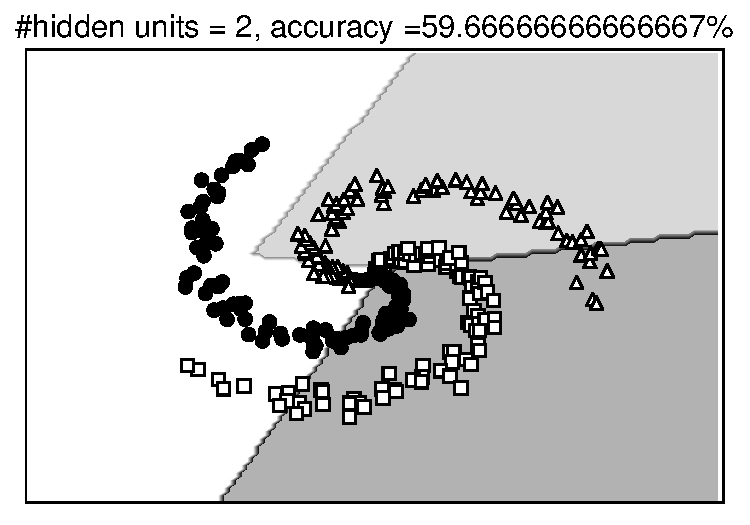
\includegraphics[width=0.99\linewidth]{ebookML_src/src/mlp/ex_res2.pdf}
    \caption{}
    % \label{fig:subim1}
    \end{subfigure}
    \begin{subfigure}{0.45\textwidth}
    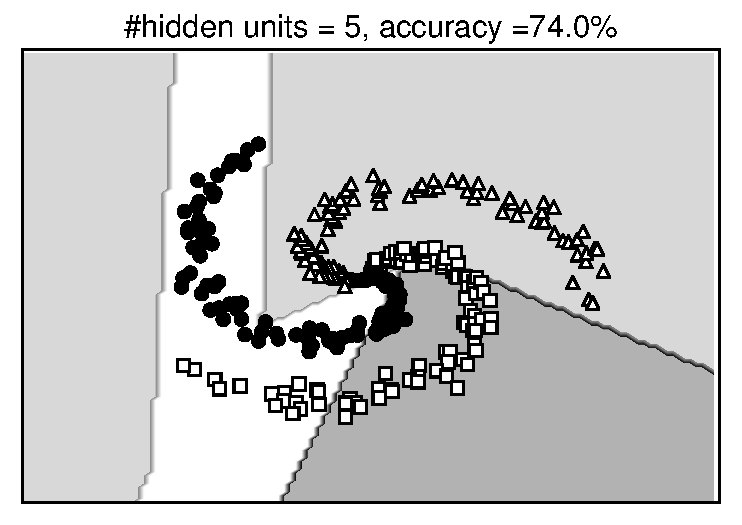
\includegraphics[width=0.99\linewidth]{ebookML_src/src/mlp/ex_res5.pdf}
    \caption{}
    % \label{fig:subim2}
    \end{subfigure}

    \begin{subfigure}{0.45\textwidth}
    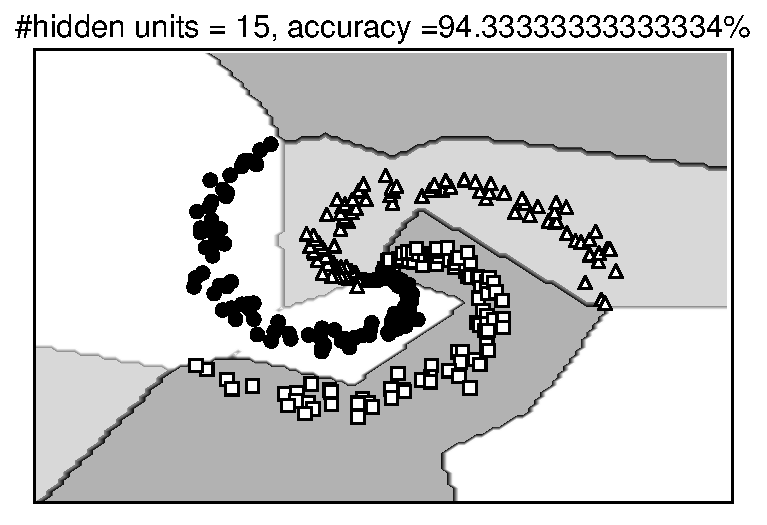
\includegraphics[width=0.99\linewidth]{ebookML_src/src/mlp/ex_res15.pdf}
    \caption{}
    % \label{fig:subim2}
    \end{subfigure}
    \begin{subfigure}{0.45\textwidth}
    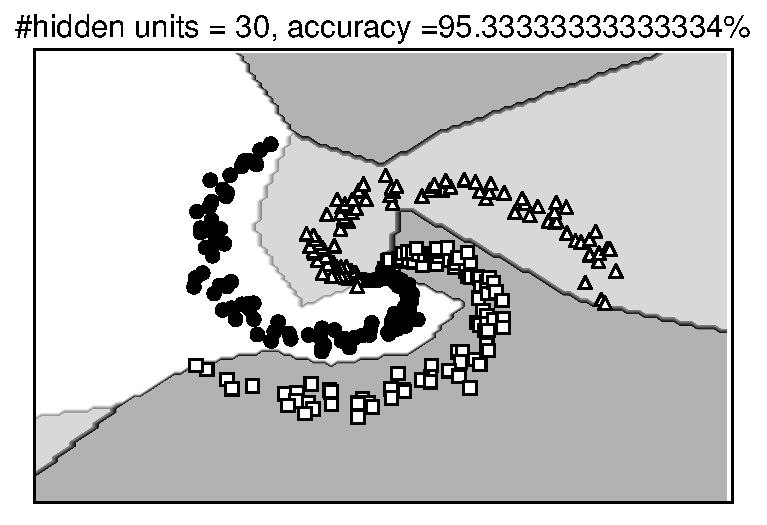
\includegraphics[width=0.99\linewidth]{ebookML_src/src/mlp/ex_res30.pdf}
    \caption{}
    % \label{fig:subim2}
    \end{subfigure}
    \caption{
     Kết quả với số lượng nút trong tầng ẩn là khác nhau.
    }
    \label{fig:14_10}
\end{figure}
% ******************************************************************************

Bằng cách thay đổi số lượng nút ẩn(biến \pythoninline{d1}) và huấn luyện lại các
mạng, chúng ta thu được các kết quả như trên Hình~\ref{fig:14_10}. Khi chỉ có
hai nút ẩn, các đường ranh giới vẫn gần như đường thẳng, kết quả là có tới 40\%
số điểm dữ liệu trong tập huấn luyện bị phân loại lỗi. Khi lượng nút ẩn là năm,
độ chính xác được cải thiện thêm khoảng 15\%, tuy nhiên, các đường ranh giới vẫn
chưa thực sự tốt. Nếu tiếp tục tăng số lượng nút ẩn, ta thấy rằng các đường ranh
giới tương đối hoàn hảo.

Có thể chứng minh được rằng với một hàm số liên tục bất kỳ $f(x)$ và một
số $\varepsilon >0$, luôn luôn tồn tại một mạng neuron mà đầu ra có dạng
$g(x)$ chỉ với một tầng ẩn (với số nút ẩn đủ lớn và hàm kích hoạt phi
tuyến phù hợp) sao cho với mọi $x, |f(x) - g(x)| < \varepsilon$. Nói cách
khác, mạng neuron có khả năng xấp xỉ hầu hết các hàm liên tục~\cite{cybenko1989approximation}.
 
Trên thực tế, việc tìm ra số lượng nút ẩn và hàm kích hoạt nói trên gần như bất
khả thi. Thay vào đó, thực nghiệm chứng minh rằng mạng neuron với nhiều tầng ẩn
kết hợp cùng các hàm kích hoạt đơn giản, ví dụ ReLU, có khả năng xấp xỉ dữ liệu
tốt hơn. Tuy nhiên, khi số lượng tầng ẩn lớn lên, số lượng trọng số cần tối ưu
cũng lớn theo và mô hình trở nên phức tạp. Sự phức tạp này ảnh hưởng tới hai
khía cạnh. Thứ nhất, tốc độ tính toán sẽ chậm đi rất nhiều. Thứ hai, nếu mô hình
quá phức tạp, nó có thể biểu diễn rất tốt dữ liệu huấn luyện, nhưng có thể không
biểu diễn tốt dữ liệu kiểm tra. Đây chính là hiện tượng quá khớp.

Vậy có các kỹ thuật nào giúp tránh quá khớp cho mạng neuron đa tầng?
Ngoài kỹ thuật xác thực chéo, chúng ta quan tâm hơn tới các phương pháp
kiểm soát. Kỹ thuật phổ biến nhất được dùng để
tránh quá khớp là \textit{suy giảm trọng số} (weight decay) hoặc dropout. 

\section{Suy giảm trọng số}
\index{suy giảm trọng số -- weight decay}
Với suy giảm trọng số, hàm mất mát sẽ được cộng thêm một đại lượng kiểm soát có
dạng:
\begin{equation*} 
\lambda R(\mathbf{W}) = \lambda \sum_{l=1}^L \|\mathbf{W}^{(l)}\|_F^2 
\end{equation*} 
tức tổng bình phương Frobenius norm của tất cả các ma trận trọng số. Chú ý rằng khi
làm việc với mạng neuron đa tầng, hệ số điều chỉnh hiếm khi được kiểm soát. Đây cũng là lý
do vì sao nên tách rời ma trận trọng số và vector điều chỉnh khi làm việc với mạng neuron
đa tầng. Việc tối thiểu hàm mất mát mới (với số hạng kiểm soát) sẽ khiến cho
thành phần của các vector trọng số $\bW^{(l)}$ không quá lớn, thậm chí nhiều thành
phần sẽ gần với không. Điều này dẫn đến việc có nhiều nút ẩn vẫn an toàn vì phần
lớn trong đó gần với không.

Tiếp theo, chúng ta sẽ làm một ví dụ khác trong không gian hai chiều. Lần này,
chúng ta sẽ sử dụng thư viện scikit-learn.




\begin{lstlisting}[language=Python]
from __future__ import print_function 
import numpy as np 
from sklearn.neural_network import MLPClassifier
means = [[-1, -1], [1, -1], [0, 1]]
cov = [[1, 0], [0, 1]]
N = 20
X0 = np.random.multivariate_normal(means[0], cov, N)
X1 = np.random.multivariate_normal(means[1], cov, N)
X2 = np.random.multivariate_normal(means[2], cov, N)

X = np.concatenate((X0, X1, X2), axis = 0)
y = np.asarray([0]*N + [1]*N + [2]*N)

alpha = 1e-1 # regularization parameter 
clf = MLPClassifier(solver='lbfgs', alpha=alpha, hidden_layer_sizes=(100))
clf.fit(X, y)
y_pred = clf.predict(X) 
acc = 100*np.mean(y_pred == y)
print('training accuracy: %.2f %%' % acc)
\end{lstlisting}
\kq
\begin{lstlisting}
training accuracy: 100.00 %
\end{lstlisting}

Trong đoạn code trên, thuộc tính \pythoninline{alpha} chính là tham số
kiểm soát $\lambda$. \pythoninline{alpha} càng lớn sẽ khiến thành phần trong các ma
trận trọng số càng nhỏ. Thuộc tính \pythoninline{hidden_layer_sizes} chính là số
lượng nút trong mỗi tầng ẩn. Nếu có nhiều tầng ẩn, chẳng hạn
hai với số nút ẩn lần lượt là 10 và 100, ta cần khai báo
\pythoninline{hidden_layer_sizes=(10, 100)}. Hình~\ref{fig:14_11} minh hoạ ranh
giới giữa các lớp tìm được với các giá trị \pythoninline{alpha} khác nhau, tức
mức độ kiểm soát khác nhau. Khi \pythoninline{alpha} nhỏ cỡ 0.01, ranh
giới tìm được trông không tự nhiên và vùng xác định lớp màu xám nhạt hơn (chứa các điểm tam giác) không được
liên tục. Mặc dù độ chính xác trên tập huấn luyện này là 100\%, ta có thể quan
sát thấy rằng quá khớp đã xảy ra. Với \pythoninline{alpha = 0.1}, kết quả cho
thấy vùng nền của các lớp đã liên tục, nhưng quá khớp vẫn xảy ra.
Khi \pythoninline{alpha} cao hơn, độ chính xác giảm xuống nhưng các đường
ranh giới tự nhiên hơn. Bạn đọc có thể thay đổi các giá trị \pythoninline{alpha}
trong mã nguồn (\url{https://goo.gl/czxrSf}) và quan sát các hiện tượng xảy
ra. Đặc biệt, khi \pythoninline{alpha = 100}, độ chính xác còn 33.33\%. Tại sao
lại như vậy? Hy vọng bạn đọc có thể tự trả lời được. 

% ******************************************************************************
\begin{figure}[t]
    \begin{subfigure}{0.45\textwidth}
    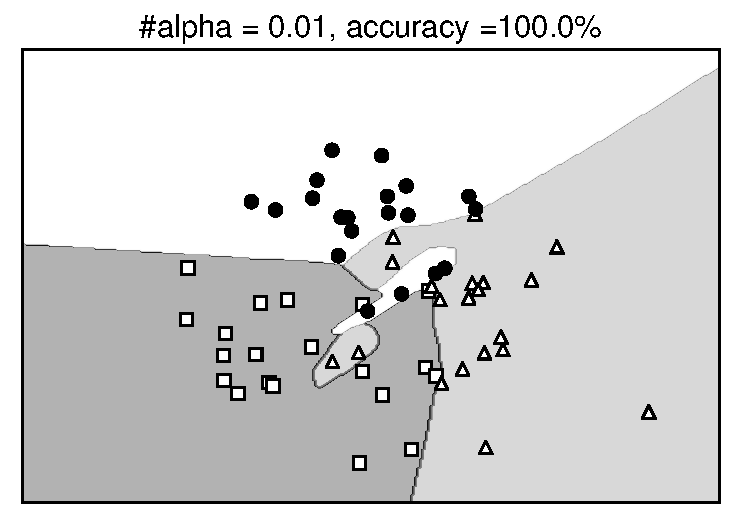
\includegraphics[width=0.99\linewidth]{ebookML_src/src/mlp/nn_overfitting_001.pdf}
    \caption{}
    % \label{fig:subim1}
    \end{subfigure}
    \begin{subfigure}{0.45\textwidth}
    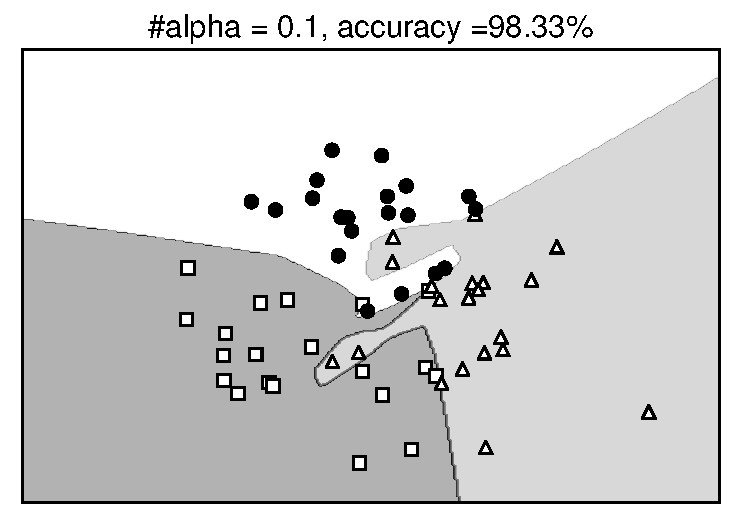
\includegraphics[width=0.99\linewidth]{ebookML_src/src/mlp/nn_overfitting_01.pdf}
    \caption{}
    % \label{fig:subim2}
    \end{subfigure}

    \begin{subfigure}{0.45\textwidth}
    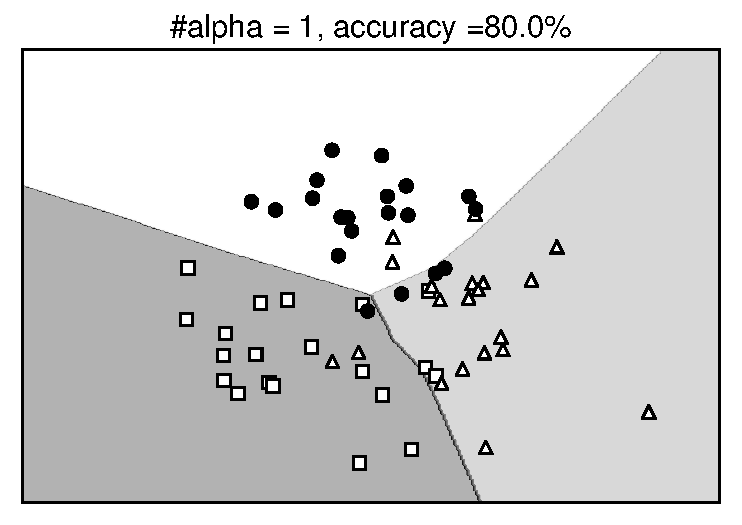
\includegraphics[width=0.99\linewidth]{ebookML_src/src/mlp/nn_overfitting_1.pdf}
    \caption{}
    % \label{fig:subim2}
    \end{subfigure}
    \begin{subfigure}{0.45\textwidth}
    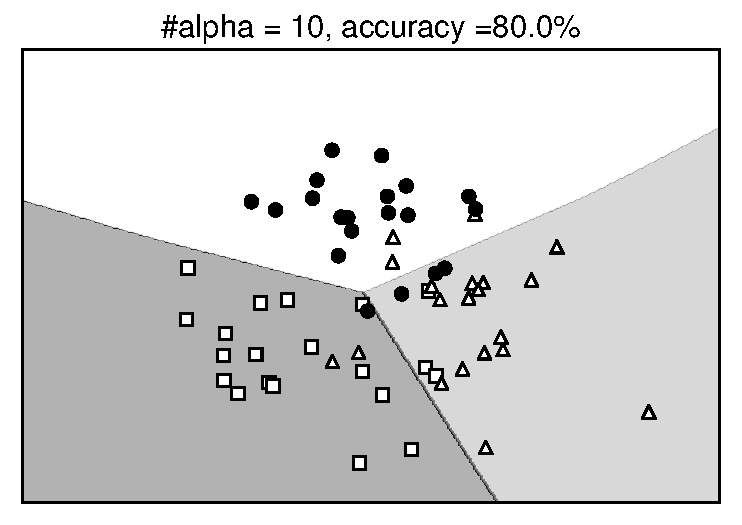
\includegraphics[width=0.99\linewidth]{ebookML_src/src/mlp/nn_overfitting_10.pdf}
    \caption{}
    % \label{fig:subim2}
    \end{subfigure}
    \caption{
     Kết quả với số nút ẩn khác nhau.
    }
    \label{fig:14_11}
\end{figure}
% ******************************************************************************


  % % \subsection{Kết quả}
% Như vậy hàm mất mát giảm dần khi số vòng lặp tăng lên. Bây giờ chúng ta cùng áp dụng ngược network này vào phân loại \textit{dữ liệu training}: 
 
 
% \begin{lstlisting}[language=Python]
% Z1 = np.dot(W1.T, X) + b1 
% A1 = np.maximum(Z1, 0) 
% Z2 = np.dot(W2.T, A1) + b2 
% predicted_class = np.argmax(Z2, axis=0) 
% print('training accuracy: %.2f %%' % (100*np.mean(predicted_class == y))) 
% \end{lstlisting}
 
%     training accuracy: 99.33 % 
 
% Vậy là trong 300 điểm, chỉ có 2 điểm bị phân loại sai! Hình \ref{fig:14_9} minh hoạ \textit{khu vực} của mỗi class: 
 
% \begin{figure}[t]
%      % caption on side     
%      \floatbox[{\capbeside\thisfloatsetup{capbesideposition={right,top},capbesidewidth=6cm}}]{figure}[\FBwidth]
%      {\caption{ 
%      Kết quả khi sử dụng một tầng ẩn với 100 units.
%      }
%      \label{fig:14_9}}
%      { % figure here
%      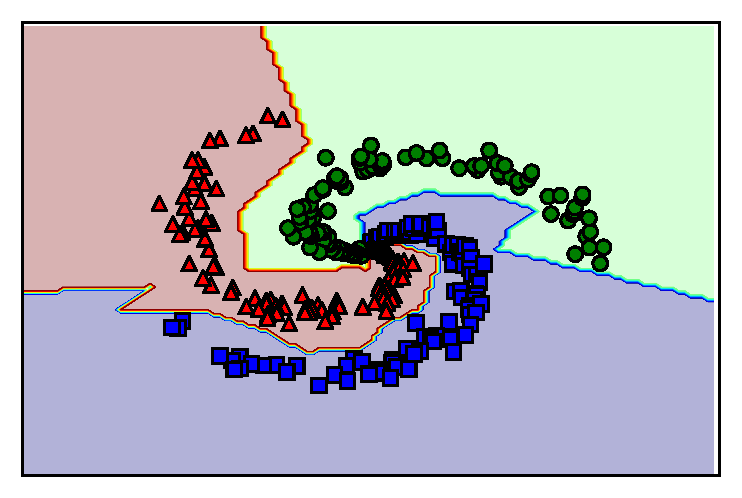
\includegraphics[width=.5\textwidth]{ebookML_src/src/mlp/ex_res32.pdf}
%      }
% %  \end{figure}
  
% Hai điểm bị phân loại sai có lẽ nằm gần khu vực trung tâm. 
 
% Vậy là chỉ thêm 1 tầng ẩn, Neural Network đã có thể xây dựng được boundary \textit{phi tuyến}. Kết luận đầu tiên ở đây là khả năng biểu diễn của MLP tốt hơn rất nhiều so với 1-layer Neural Network. 
 
 
 
% Kết quả bên trên được thực hiện khi số lượng units trong hidden layer là \pythoninline{d1 = 100}. Chúng ta thử thay đổi giá trị này bởi \pythoninline{d1 = 5, 10, 15, 20} xem kết quả khác nhau như thế nào. Kết quả được minh hoạ trong Hình \ref{fig:14_10}.
 

 
% Có một vài nhận xét như sau: 
% \begin{itemize}
% \item Khi số lượng nút ẩn  tăng lên, độ chính xác của mô hình tạo được cũng tăng lên. 
 
% \item Với \pythoninline{d1 = 5}, đường phân định giữa ba classes gần như là đường thẳng. 
 
% \item Với \pythoninline{d1 = 15}, mặc dù kết quả đã đạt 99.33\%, vẫn có một vùng đỏ nhỏ nằm giữa nhánh màu lục và màu lam, và một vùng màu lam khá lớn giữa màu đỏ và lục. Khi một điểm dữ liệu test rơi vào những vùng này, nó sẽ bị phân loại sai. 
 
% \item Với \pythoninline{d1 = 20}, kết quả nhận được đã tương đối giống với \pythoninline{d1 = 100}. Mặc dù các đường boundary không được trơn tru cho lắm. 
 
% \end{itemize}
 
% \section{Thảo luận}
% \begin{itemize}
% \item \href{http://www.dartmouth.edu/~gvc/Cybenko_MCSS.pdf}{Người ta đã chứng minh được rằng}, với một hàm số liên tục bất kỳ $f(x)$ và một số $\varepsilon >0$, luôn luôn tồn tại một Neural Network với predicted output có dạng $g(x)$ với một hidden layer (với số hidden units đủ lớn và \textit{nonlinear} activation function phù hợp) sao cho với mọi $x, \|f(x) - g(x)\| < \varepsilon$. Nói một cách khác, Neural Network có khả năng xấp xỉ bất kỳ hàm liên tục nào. 
 
% \item Trên thực tế, việc tìm ra số lượng hidden units và \textit{nonlinear} activation function nói trên nhiều khi bất khả thi. Thay vào đó, thực nghiệm chứng minh rằng Neural Networks với nhiều hidden layers kết hợp với các \textit{nonlinear} activation function (đơn giản như ReLU) có khả năng xấp xỉ (khả năng biểu diễn) training data tốt hơn. 
 
% \item Khi số lượng hidden layers lớn lên, số lượng hệ số cần tối ưu cũng lớn lên và mô hình sẽ trở nên phức tạp. Sự phức tạp này ảnh hưởng tới hai khia cạnh. Thứ nhất, tốc độ tính toán sẽ bị chậm đi rất nhiều. Thứ hai, nếu mô hình quá phức tạp, nó có thể biểu diễn rất tốt training data, nhưng lại không biểu diễn tốt test data. Hiện tượng này gọi là \href{https://en.wikipedia.org/wiki/Overfitting}{Overfitting}, tôi sẽ trình bày trong bài sau. 
 
 
% \item Đây là bài cuối cùng trong chuỗi bài về Neural Networks. Viết một bài về Deep Learning sẽ tốn thời gian hơn rất nhiều, trong 1 tuần tôi không đủ khả năng hoàn thành được. Bài tiếp theo tôi sẽ nói về \href{https://en.wikipedia.org/wiki/Overfitting}{Overfitting}, sau đó chuyển sang một phương pháp classification rất phổ biến khác: \href{https://en.wikipedia.org/wiki/Support_vector_machine}{Support Vector Machine}. 
 
% \item Về backpropagation, có rất nhiều điều phải nói nữa. Nếu có thể, tôi xin phép được trình bày sau. Bài này cũng đã đủ dài. 
 
%  \end{itemize} 
 
\newpage 
\section{Đọc thêm}
\begin{enumerate}
    \item \textit{Neural Networks: Setting up the Architecture}, Andrej Karpathy
    (\url{https://goo.gl/rfzCVK}). 

    \item \textit{Neural Networks, Case study}, Andrej Karpathy
    (\url{https://goo.gl/3ihCxL}).
 
    \item \textit{Lecture Notes on Sparse Autoencoders}, Andrew Ng
    (\url{https://goo.gl/yTgtLe}).
 
    \item \textit{Yes you should understand backprop} (\url{https://goo.gl/8B3h1b}). 
 
    \item \textit{Backpropagation, Intuitions}, Andrej Karpathy
    (\url{https://goo.gl/fjHzNV}).
 
    \item \textit{How the backpropagation algorithm works}, Michael Nielsen
    (\url{https://goo.gl/mwz2kU}). 
\end{enumerate}



 
